\documentclass{article}
\usepackage{xcolor}
\usepackage{tcolorbox}
\usepackage{amsmath}
\usepackage{fancyhdr}
\usepackage{titlesec}
\usepackage{geometry}
\usepackage{sectsty}
\usepackage{minted}
\usepackage{tabularx}
\usepackage{booktabs}
\usepackage{mathptmx}
\usepackage{graphicx}
\usepackage{hyperref}
\usepackage{enumitem}
\usepackage{tikz}
\usetikzlibrary{shapes.geometric, arrows.meta, positioning, fit, backgrounds, calc}
\usepackage{pgfplots}
\pgfplotsset{compat=1.18}
\usepackage{caption}
\usepackage{float}

% Page layout
\geometry{margin=1in}

% Header and footer
\pagestyle{fancy}
\fancyhf{}
\fancyhead[L]{Protocol Extraction Pipeline}
\fancyhead[R]{Code Documentation}
\fancyfoot[C]{\thepage}

% Define colors
\definecolor{lightblue}{RGB}{240, 248, 255}
\definecolor{lightbeige}{RGB}{255, 250, 240}
\definecolor{lightpink}{RGB}{255, 230, 230}
\definecolor{deepred}{RGB}{128, 0, 0}
\definecolor{mygray}{RGB}{245, 245, 245}
\definecolor{darkblue}{RGB}{30, 60, 120}

% Title styling
\titleformat{\section}
  {\normalfont\Large\bfseries\color{deepred}}{\thesection}{1em}{}
\titleformat{\subsection}
  {\normalfont\large\bfseries\color{deepred}}{\thesubsection}{1em}{}
\titleformat{\subsubsection}
  {\normalfont\normalsize\bfseries\color{deepred}}{\thesubsubsection}{1em}{}

\sectionfont{\color{deepred}}
\subsectionfont{\color{deepred}}
\subsubsectionfont{\color{deepred}}

% Hyperref styling
\hypersetup{
    colorlinks=true,
    linkcolor=darkblue,
    citecolor=darkblue,
    urlcolor=darkblue,
}

% Title page command
\newcommand{\titlepagecontent}{
    \begin{titlepage}
        \begin{center}
            \IfFileExists{AUB.png}{%
                \includegraphics[width=0.4\textwidth]{AUB.png}\\[1.5cm]%
            }{\vspace*{1.5cm}}

            {\huge\bfseries Protocol Extraction Pipeline}\\[0.5cm]

            {\Large\bfseries Code Documentation}\\[0.4cm]
            \textit{\large An LLM-Based System for Constructing Protocol Knowledge
            Graphs from Emergency Response PDFs}\\[0.4cm]

            \vspace{0.8cm}
            \makebox[\textwidth]{\textcolor{deepred}{\rule{0.7\textwidth}{1pt}}} \\[0.4cm]
            \makebox[\textwidth]{\textcolor{deepred}{\rule{0.5\textwidth}{1pt}}} \\[0.4cm]
            \makebox[\textwidth]{\textcolor{deepred}{\rule{0.3\textwidth}{1.5pt}}}

            \vspace{5cm}
            {\Large\bfseries Safaa Salman}\\[0.2cm]
            \textit{American University of Beirut}\\[1cm]

            \vfill
            {\large May, 2026}
            \vspace{1cm}
        \end{center}
    \end{titlepage}
}

% Important Note box
\newtcolorbox{importantnote}[1][]{
    colback=lightbeige, colframe=deepred, fonttitle=\bfseries,
    title=Important Note, sharp corners, boxrule=0.2mm, width=\textwidth, #1
}

% Concept boxes
\newtcolorbox{conceptbox}[1][]{
    colback=lightblue, colframe=darkblue, fonttitle=\bfseries,
    boxrule=0.2mm, sharp corners, width=\textwidth, #1
}
\newtcolorbox{codeconceptbox}[1][]{
    colback=lightbeige, colframe=lightbeige,
    fonttitle=\bfseries\color{deepred}, boxrule=0.2mm,
    sharp corners, width=\textwidth, title=#1
}
\newtcolorbox{componentbox}[1][]{
    colback=lightblue, colframe=darkblue, fonttitle=\bfseries,
    boxrule=0.2mm, sharp corners, width=\textwidth, #1
}

% Begin document
\begin{document}

\titlepagecontent

\tableofcontents
\newpage

% =====================================================================
\section{Project Overview}
\label{sec:overview}

This document describes the implementation of a pipeline that extracts
structured protocol graphs from emergency response PDF documents. Each
extracted protocol is a directed graph in which the nodes represent
procedural steps or decision points and the edges represent ordering
and conditional branching. The pipeline takes a PDF as input and
produces, for every detected protocol, a JSON graph that conforms to a
fixed schema and links every node back to its source page and text.

\subsection{Research Question}

\begin{conceptbox}
\textit{Can the procedural structure of emergency response protocols be
extracted from PDF documents reliably enough to support a protocol
centric knowledge graph?}
\end{conceptbox}

The work focuses on the procedural layer first. The graph captures the
ordering of steps and the conditions under which the protocol branches.
A semantic enrichment layer that identifies roles, equipment and
hazards is provided as an optional second pass on top of the extracted
graphs.

\subsection{Target Documents}

The pipeline is exercised on two complete documents.

\begin{table}[H]
\centering
\begin{tabularx}{\textwidth}{l c c X}
\toprule
\textbf{Document} & \textbf{Pages} & \textbf{Protocols} & \textbf{Description} \\
\midrule
IRPG 2025 & 140 & 49 extracted from 99 sections & NWCG Incident Response Pocket Guide. United States wildland fire and emergency medical protocols. \\
\addlinespace
VIC Bushfire Handbook & 100 & 30 extracted from 98 sections & Victorian (Australia) emergency management policies and procedures. \\
\bottomrule
\end{tabularx}
\caption{Source documents used for development and evaluation.}
\label{tab:source-docs}
\end{table}

A total of 79 protocol graphs are produced across the two documents
with no extraction errors. Five of the IRPG protocols (CPR, Burn
Injuries, Patient Assessment, Risk Management and Multi Casualty
Triage) are manually annotated as gold standards and serve as the
quantitative evaluation set.

\subsection{Output of the Pipeline}

For every detected protocol the pipeline produces a JSON file
conforming to a fixed schema. The schema is small enough to fit in a
single listing.

\begin{tcolorbox}[colback=mygray, colframe=mygray, sharp corners, boxrule=0pt]
\begin{minted}[fontsize=\small, breaklines]{json}
{
  "protocol_id": "cpr",
  "title": "CPR",
  "source_pdf": "IRPG-2025.pdf",
  "pages": [127],
  "protocol_type": "decision_tree",
  "extraction_confidence": 0.85,
  "cross_references": ["Patient Assessment"],
  "nodes": [
    { "id": "n1", "type": "start",
      "text": "Ensure scene safety",
      "evidence": { "page": 127,
                    "source_text": "Ensure scene safety..." } }
  ],
  "edges": [
    { "from": "n1", "to": "n2" },
    { "from": "n3", "to": "n4",
      "condition": "Yes (breathing)" }
  ]
}
\end{minted}
\end{tcolorbox}

Each node carries a type drawn from the set
\{\texttt{start}, \texttt{end}, \texttt{action}, \texttt{decision}\}
and an evidence block that records the page and source text the node
came from. Each edge optionally carries a condition label describing
the branch it represents. The schema is enforced as a JSON Schema
document and is the single contract that every component in the
pipeline reads from or writes to.

Figure~\ref{fig:cpr-example} shows what the schema looks like once it
is rendered as a graph. The example is an abbreviated view of the
gold standard CPR protocol from IRPG 2025. The full annotation has
seventeen nodes and nineteen edges; three further decision points
(spinal injury, barrier device availability and the inner CPR loop)
are omitted from the figure for clarity but are present in
\texttt{evaluation/gold/cpr\_01.json}.

\begin{figure}[H]
\centering
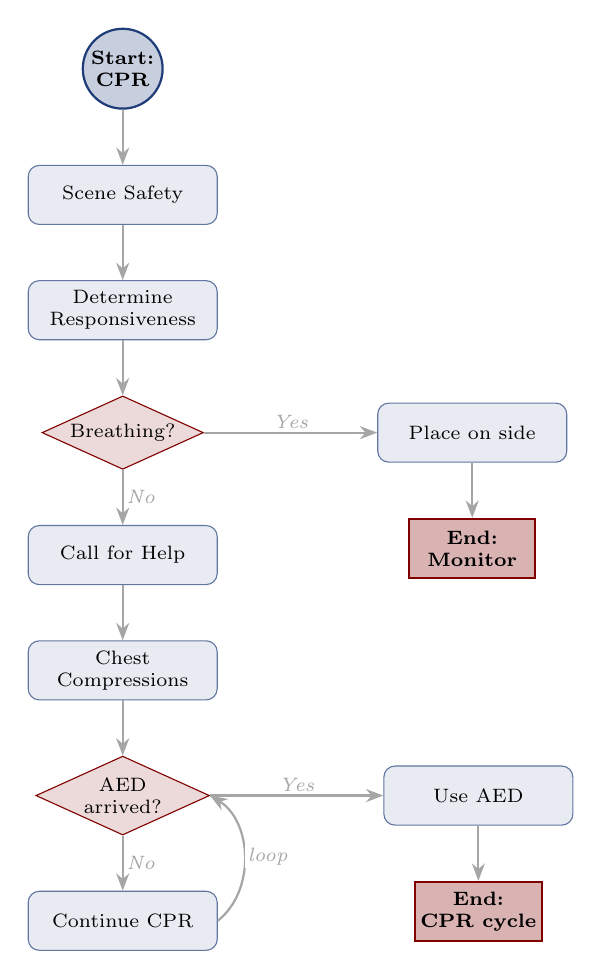
\begin{tikzpicture}[
    node distance=0.7cm and 1.4cm,
    startnode/.style={draw=darkblue, thick, circle, fill=darkblue!25,
                      minimum size=1cm, inner sep=1pt,
                      font=\scriptsize\bfseries, align=center},
    endnode/.style={draw=deepred, thick, rectangle, fill=deepred!30,
                    minimum width=1.6cm, minimum height=0.75cm,
                    inner sep=2pt, font=\scriptsize\bfseries,
                    align=center},
    actionnode/.style={draw=darkblue!70, rounded corners=4pt,
                       fill=darkblue!10,
                       minimum width=2.4cm, minimum height=0.75cm,
                       inner sep=2pt, font=\scriptsize, align=center},
    decisionnode/.style={draw=deepred, diamond, aspect=2.2,
                         fill=deepred!15, inner sep=1pt,
                         font=\scriptsize, align=center},
    arr/.style={-{Stealth[length=2.2mm]}, thick, color=gray!70},
    cond/.style={font=\scriptsize\itshape, fill=white, inner sep=1pt},
]
    \node[startnode] (n1) {Start: \\ CPR};
    \node[actionnode, below=of n1] (n2) {Scene Safety};
    \node[actionnode, below=of n2] (n3) {Determine\\Responsiveness};
    \node[decisionnode, below=of n3] (n4) {Breathing?};
    \node[actionnode, right=2.2cm of n4] (n6) {Place on side};
    \node[endnode, below=of n6] (n7) {End:\\Monitor};
    \node[actionnode, below=of n4] (n5) {Call for Help};
    \node[actionnode, below=of n5] (n9) {Chest\\Compressions};
    \node[decisionnode, below=of n9] (n15) {AED\\arrived?};
    \node[actionnode, right=2.2cm of n15] (n16) {Use AED};
    \node[endnode, below=of n16] (n17) {End:\\CPR cycle};
    \node[actionnode, below=of n15] (n14) {Continue CPR};

    \draw[arr] (n1) -- (n2);
    \draw[arr] (n2) -- (n3);
    \draw[arr] (n3) -- (n4);
    \draw[arr] (n4) -- node[cond, above]{Yes} (n6);
    \draw[arr] (n4) -- node[cond, right]{No} (n5);
    \draw[arr] (n6) -- (n7);
    \draw[arr] (n5) -- (n9);
    \draw[arr] (n9) -- (n15);
    \draw[arr] (n15) -- node[cond, above]{Yes} (n16);
    \draw[arr] (n15) -- node[cond, right]{No} (n14);
    \draw[arr] (n16) -- (n17);
    \draw[arr] (n14.east) to[bend right=55] node[cond, right]{loop} (n15.east);
\end{tikzpicture}
\caption{Abbreviated view of the gold standard CPR protocol graph.
The start node is a dark blue circle, action nodes are light blue
rounded rectangles, decision nodes are deep red diamonds and end
nodes are deep red rectangles. Edge labels carry the condition under
which the branch is taken. \texttt{visualize.py} and the interactive
viewer use the same node shapes with a brighter palette
(green / blue / orange / red).}
\label{fig:cpr-example}
\end{figure}

\subsection{What This Document Covers}

The remainder of this document is organised in two parts.
Section~\ref{sec:architecture} explains the pipeline architecture and
the rationale behind each design decision, including the diagrams that
describe the flow of data through the system. The code documentation
that follows describes each source file, the public functions it
exposes, and how the entry point scripts tie the pieces together.

% =====================================================================
\section{Architecture and Design Decisions}
\label{sec:architecture}

This section walks through the pipeline stage by stage and explains
why each component is built the way it is. The exposition follows the
order in which a PDF travels through the system rather than the order
in which the code was written.

\subsection{Pipeline at a Glance}

The pipeline is organised into seven stages. Stages one through three
prepare the document, stage four performs the extraction itself, stages
five and six enforce quality, and stage seven persists the results.
Figure~\ref{fig:pipeline} shows the flow.

\begin{figure}[H]
\centering
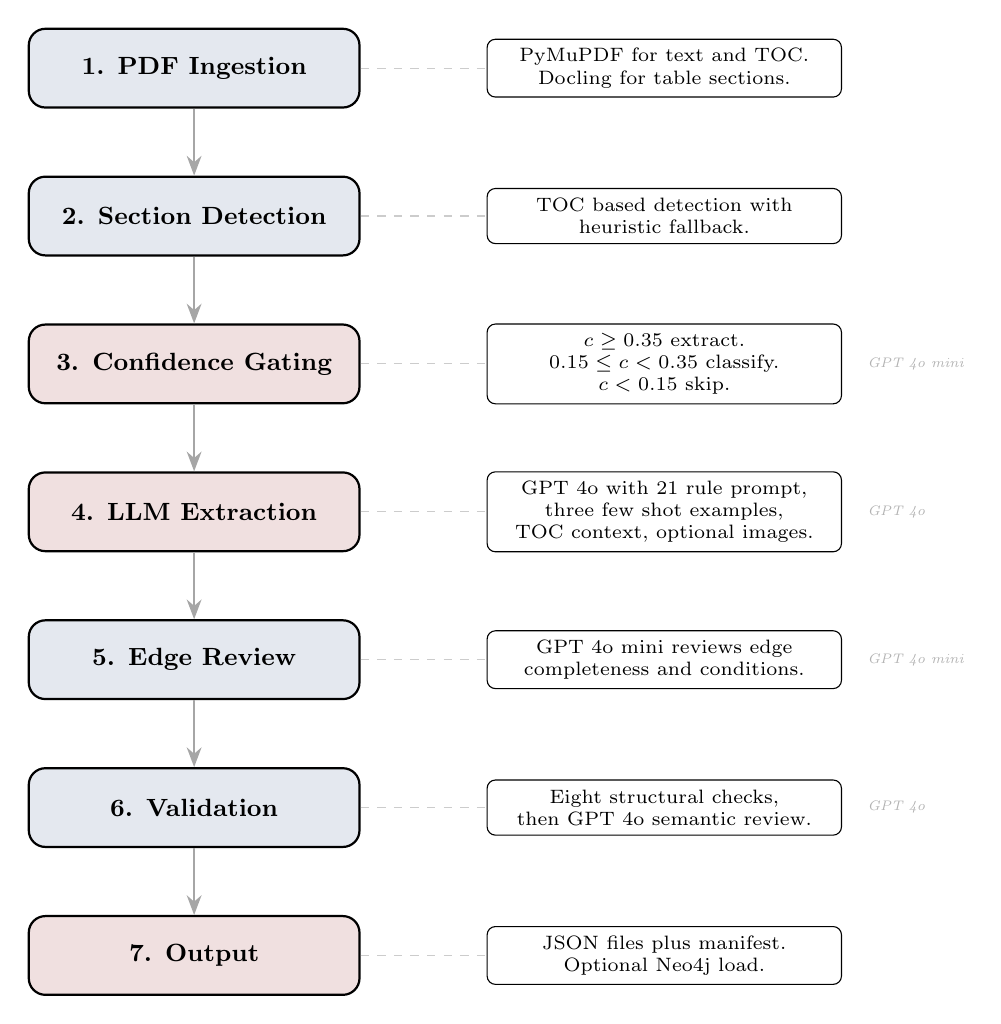
\begin{tikzpicture}[
    node distance=0.85cm and 1.6cm,
    stage/.style={draw, rounded corners=6pt, minimum width=4.2cm,
                  minimum height=1cm, align=center, font=\small\bfseries,
                  thick},
    substage/.style={draw, rounded corners=3pt, minimum width=4.5cm,
                     minimum height=0.7cm, align=center, font=\scriptsize,
                     thin, fill=white},
    arrow/.style={-{Stealth[length=2.5mm]}, thick, color=gray!70},
    lbl/.style={font=\tiny\itshape, color=gray!60},
]
    \node[stage, fill=darkblue!12] (ingest) {1. PDF Ingestion};
    \node[stage, fill=darkblue!12, below=of ingest] (detect) {2. Section Detection};
    \node[stage, fill=deepred!12, below=of detect] (gate) {3. Confidence Gating};
    \node[stage, fill=deepred!12, below=of gate] (extract) {4. LLM Extraction};
    \node[stage, fill=darkblue!12, below=of extract] (review) {5. Edge Review};
    \node[stage, fill=darkblue!12, below=of review] (validate) {6. Validation};
    \node[stage, fill=deepred!12, below=of validate] (output) {7. Output};

    \draw[arrow] (ingest) -- (detect);
    \draw[arrow] (detect) -- (gate);
    \draw[arrow] (gate) -- (extract);
    \draw[arrow] (extract) -- (review);
    \draw[arrow] (review) -- (validate);
    \draw[arrow] (validate) -- (output);

    \node[substage, right=1.6cm of ingest] (s1)
        {PyMuPDF for text and TOC.\\Docling for table sections.};
    \node[substage, right=1.6cm of detect] (s2)
        {TOC based detection with\\heuristic fallback.};
    \node[substage, right=1.6cm of gate] (s3)
        {$c \geq 0.35$ extract.\\$0.15 \leq c < 0.35$ classify.\\$c < 0.15$ skip.};
    \node[substage, right=1.6cm of extract] (s4)
        {GPT 4o with 21 rule prompt,\\three few shot examples,\\TOC context, optional images.};
    \node[substage, right=1.6cm of review] (s5)
        {GPT 4o mini reviews edge\\completeness and conditions.};
    \node[substage, right=1.6cm of validate] (s6)
        {Eight structural checks,\\then GPT 4o semantic review.};
    \node[substage, right=1.6cm of output] (s7)
        {JSON files plus manifest.\\Optional Neo4j load.};

    \draw[gray!40, dashed] (ingest.east) -- (s1.west);
    \draw[gray!40, dashed] (detect.east) -- (s2.west);
    \draw[gray!40, dashed] (gate.east) -- (s3.west);
    \draw[gray!40, dashed] (extract.east) -- (s4.west);
    \draw[gray!40, dashed] (review.east) -- (s5.west);
    \draw[gray!40, dashed] (validate.east) -- (s6.west);
    \draw[gray!40, dashed] (output.east) -- (s7.west);

    \node[lbl, right=0.2cm of s3] {GPT 4o mini};
    \node[lbl, right=0.2cm of s4] {GPT 4o};
    \node[lbl, right=0.2cm of s5] {GPT 4o mini};
    \node[lbl, right=0.2cm of s6] {GPT 4o};
\end{tikzpicture}
\caption{Pipeline stages and the substage detail behind each. The
left column lists the stage. The right column summarises what runs
inside the stage and which model, if any, is used.}
\label{fig:pipeline}
\end{figure}

\subsection{Module Layout}

Figure~\ref{fig:modules} shows how the source code is laid out and how
the modules depend on each other. The dependency graph is acyclic and
every module depends on at most a small fixed set of others. The
ingestion layer at the top is the only layer that talks to PyMuPDF and
Docling. The extraction layer in the middle is the only layer that
talks to the OpenAI API. The graph layer at the bottom is the only
layer that talks to Neo4j. The entry point scripts live at the project
root and compose these layers.

\begin{figure}[H]
\centering
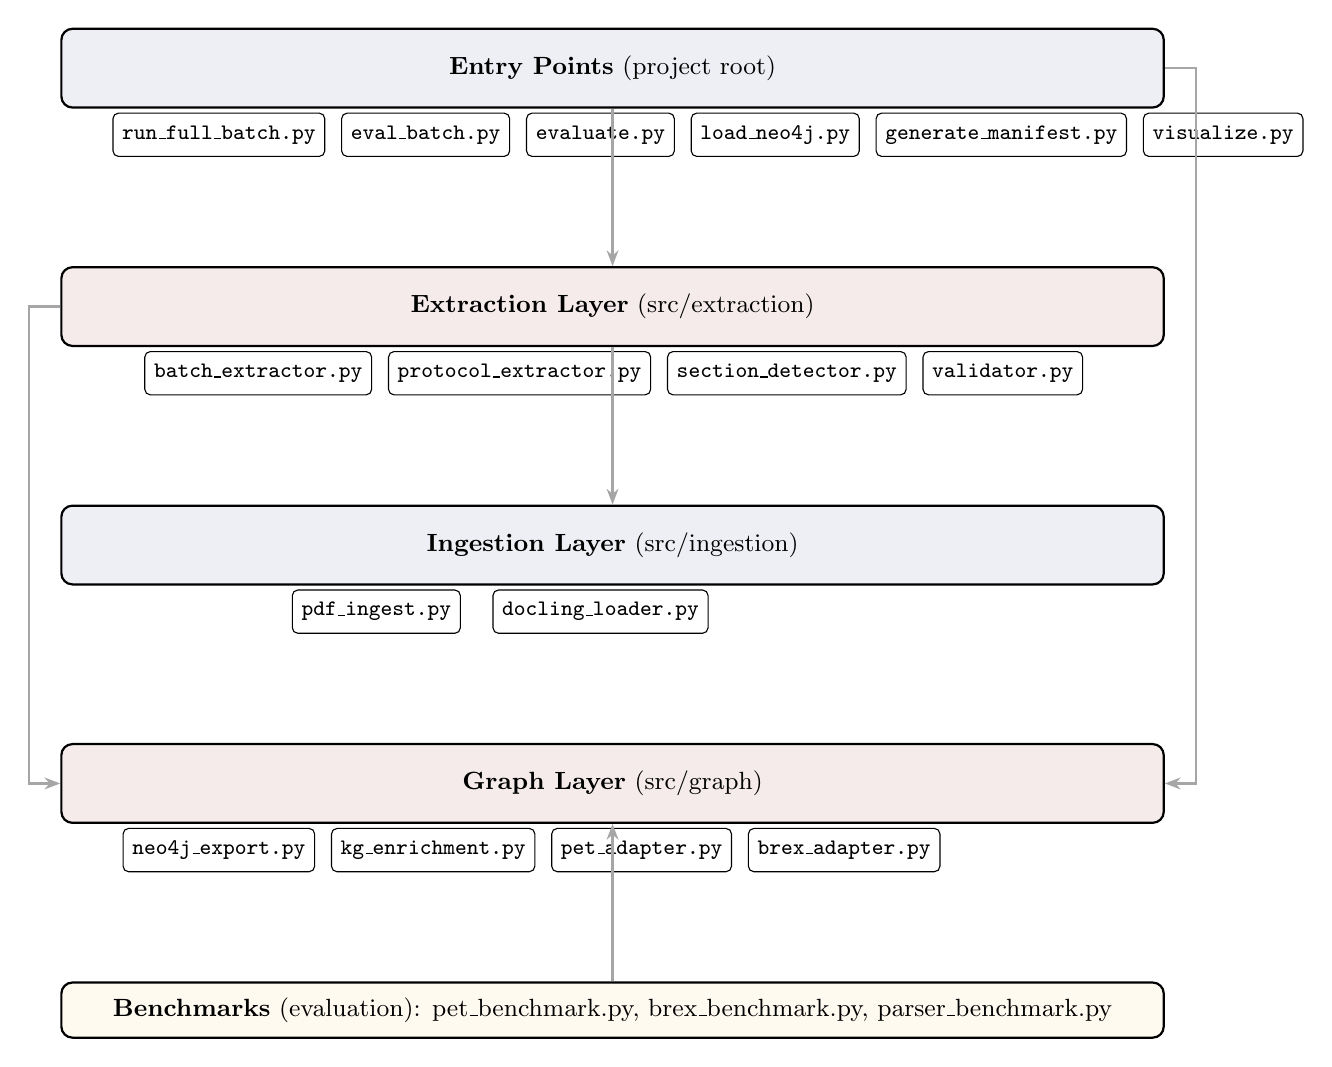
\begin{tikzpicture}[
    layer/.style={draw, rounded corners=4pt, minimum width=14cm,
                  minimum height=1cm, align=center, font=\small,
                  thick},
    mod/.style={draw, rounded corners=2pt, minimum height=0.55cm,
                align=center, font=\footnotesize\ttfamily, fill=white},
    arr/.style={-{Stealth[length=2mm]}, thick, color=gray!70},
]
    \node[layer, fill=darkblue!8]   (ent)  {\textbf{Entry Points} (project root)};
    \node[mod, below=0.05cm of ent.south, xshift=-5cm] (rfb)  {run\_full\_batch.py};
    \node[mod, right=0.2cm of rfb]                     (eb)   {eval\_batch.py};
    \node[mod, right=0.2cm of eb]                      (ev)   {evaluate.py};
    \node[mod, right=0.2cm of ev]                      (ln)   {load\_neo4j.py};
    \node[mod, right=0.2cm of ln]                      (gm)   {generate\_manifest.py};
    \node[mod, right=0.2cm of gm]                      (vis)  {visualize.py};

    \node[layer, fill=deepred!8, below=2.0cm of ent]   (ext)  {\textbf{Extraction Layer} (src/extraction)};
    \node[mod, below=0.05cm of ext.south, xshift=-4.5cm] (be)  {batch\_extractor.py};
    \node[mod, right=0.2cm of be]                       (pe)  {protocol\_extractor.py};
    \node[mod, right=0.2cm of pe]                       (sd)  {section\_detector.py};
    \node[mod, right=0.2cm of sd]                       (vd)  {validator.py};

    \node[layer, fill=darkblue!8, below=2.0cm of ext]   (ing) {\textbf{Ingestion Layer} (src/ingestion)};
    \node[mod, below=0.05cm of ing.south, xshift=-3cm]  (pi)  {pdf\_ingest.py};
    \node[mod, right=0.4cm of pi]                       (dl)  {docling\_loader.py};

    \node[layer, fill=deepred!8, below=2.0cm of ing]    (gr)  {\textbf{Graph Layer} (src/graph)};
    \node[mod, below=0.05cm of gr.south, xshift=-5cm]   (ne)  {neo4j\_export.py};
    \node[mod, right=0.2cm of ne]                       (ke)  {kg\_enrichment.py};
    \node[mod, right=0.2cm of ke]                       (pa)  {pet\_adapter.py};
    \node[mod, right=0.2cm of pa]                       (ba)  {brex\_adapter.py};

    \node[layer, fill=lightbeige, below=2.0cm of gr, minimum height=0.7cm] (ben)
        {\textbf{Benchmarks} (evaluation): pet\_benchmark.py, brex\_benchmark.py, parser\_benchmark.py};

    \draw[arr] (ent) -- (ext);
    \draw[arr] (ext) -- (ing);
    \draw[arr] (ent.east) -- ++(0.4cm,0) |- (gr.east);
    \draw[arr] (ext.west) -- ++(-0.4cm,0) |- (gr.west);
    \draw[arr] (ben) -- (gr);
\end{tikzpicture}
\caption{Module layout and dependency direction. Arrows indicate which
layer imports from which. The ingestion layer has no internal
dependencies. The extraction layer depends only on ingestion. The
graph layer depends on nothing internal and is reused by both
benchmarks and entry points.}
\label{fig:modules}
\end{figure}

\subsection{Stage 1. PDF Ingestion}

The first stage reads a PDF and produces an in memory representation
that downstream stages can query without ever touching the original
file again. The default loader uses PyMuPDF and exposes per page text
blocks with bounding boxes, page level tables, the table of contents
and a flag that records whether the PDF is native or scanned. A second
loader based on IBM Docling is invoked only for sections whose format
hint is \texttt{table}.

\begin{importantnote}
The choice of two loaders is deliberate. PyMuPDF is fast and accurate
for free flowing text but flattens tables into linear strings.
Docling is slower but uses the DocLayNet layout model and TableFormer
to preserve row and column structure as Markdown. Routing sections by
their format hint avoids paying the Docling cost on text heavy pages
while still recovering table structure where it matters.
\end{importantnote}

\subsection{Stage 2. Section Detection}

A document like IRPG 2025 contains 99 sections, only some of which are
actual protocols. The section detector is the component that decides
which page ranges should be considered candidates for extraction. Two
signals are used.

\begin{enumerate}[leftmargin=2em]
    \item \textbf{Table of contents.} If the PDF carries a TOC, the
    detector walks it and treats every leaf entry as a candidate
    section with a known title, start page and end page. The TOC also
    yields the parent category, which is later passed to the LLM as a
    breadcrumb.
    \item \textbf{Heuristic fallback.} If no TOC is present, or for
    sections inside a TOC entry that contain further protocols, the
    detector falls back to regular expression matching for headings,
    numbered steps, decision keywords and imperative verbs.
\end{enumerate}

For every candidate section the detector also assigns a format hint
drawn from the set \{\texttt{sequential}, \texttt{decision\_tree},
\texttt{table}, \texttt{hybrid}, \texttt{checklist},
\texttt{reference}\} and a confidence score in $[0, 1]$. The
confidence score is the input to the next stage.

\subsubsection{Confidence Score Composition}

The confidence assigned to a section is a sum of weighted bonuses for
the markers a real protocol typically exhibits, capped at one. Each
marker is itself a thresholded match against the section text.

\begin{align}
c &= \min\!\Big(\;
      0.25 \cdot \mathbf{1}[\text{title keyword}]
    + 0.20 \cdot \mathbf{1}[\text{numbered steps}] \notag \\
    &\quad + 0.20 \cdot \mathbf{1}[\text{decision logic}]
    + 0.10 \cdot \mathbf{1}[\text{tables}] \notag \\
    &\quad + f_{\text{length}}
    + 0.10 \cdot \mathbf{1}[\text{imperative language}]
    \;,\; 1\Big)
\end{align}

The length term $f_{\text{length}}$ is 0.15 when the section spans
between one and ten pages and 0.05 when it spans more. The indicator
flags fire only when their underlying patterns cross a count
threshold: \texttt{numbered steps} requires at least two matches of
the \texttt{NUMBERED\_STEP\_PATTERN} regular expression,
\texttt{decision logic} requires at least one match of
\texttt{DECISION\_PATTERNS} and \texttt{imperative language} requires
at least one match of \texttt{IMPERATIVE\_PATTERN}. Sections marked
\texttt{is\_protocol = false} -- because their title matches the
non protocol filter described below or because they are level one
TOC entries with children -- are forced to confidence zero and never
reach extraction.

\subsubsection{Format Hint Assignment}

The format hint is decided by a small priority cascade over the same
flags. The first matching rule wins.

\begin{enumerate}[leftmargin=2em]
    \item Tables and decisions present $\Rightarrow$ \texttt{hybrid}.
    \item Tables only $\Rightarrow$ \texttt{table}.
    \item Numbered steps and decisions $\Rightarrow$
        \texttt{decision\_tree}.
    \item Numbered steps only $\Rightarrow$ \texttt{sequential}.
    \item At least three imperative bullets and no numbered steps
        $\Rightarrow$ \texttt{checklist}.
    \item Decisions only $\Rightarrow$ \texttt{decision\_tree}.
    \item Otherwise $\Rightarrow$ \texttt{reference}.
\end{enumerate}

The \texttt{reference} hint is the typical destination for tables of
contents, glossaries and similar non procedural pages, and combines
with the low confidence score to keep them out of the extractor.

\subsubsection{Non Protocol Title Filter}

Before scoring, section titles are filtered against the
\texttt{NON\_PROTOCOL\_TITLES} regular expression, which matches the
words \emph{notes}, \emph{glossary}, \emph{index},
\emph{table of contents}, \emph{appendix}, \emph{references},
\emph{abbreviations}, \emph{acknowledgments}, \emph{foreword},
\emph{preface} and \emph{introduction}. Matching titles have
\texttt{is\_protocol} set to false and are dropped from confidence
scoring. The heuristic heading detector additionally skips PDF chrome
such as the literal \texttt{IRPG} prefix and
\texttt{Page \textbackslash d+ of \textbackslash d+} running heads.

\subsection{Stage 3. Confidence Gating}

The third stage routes each scored section into one of three buckets.
Routing the document this way rather than extracting every section
saves between 50 and 70 percent of the LLM budget without losing
extractable content. Figure~\ref{fig:gating} shows the decision flow.

\begin{figure}[H]
\centering
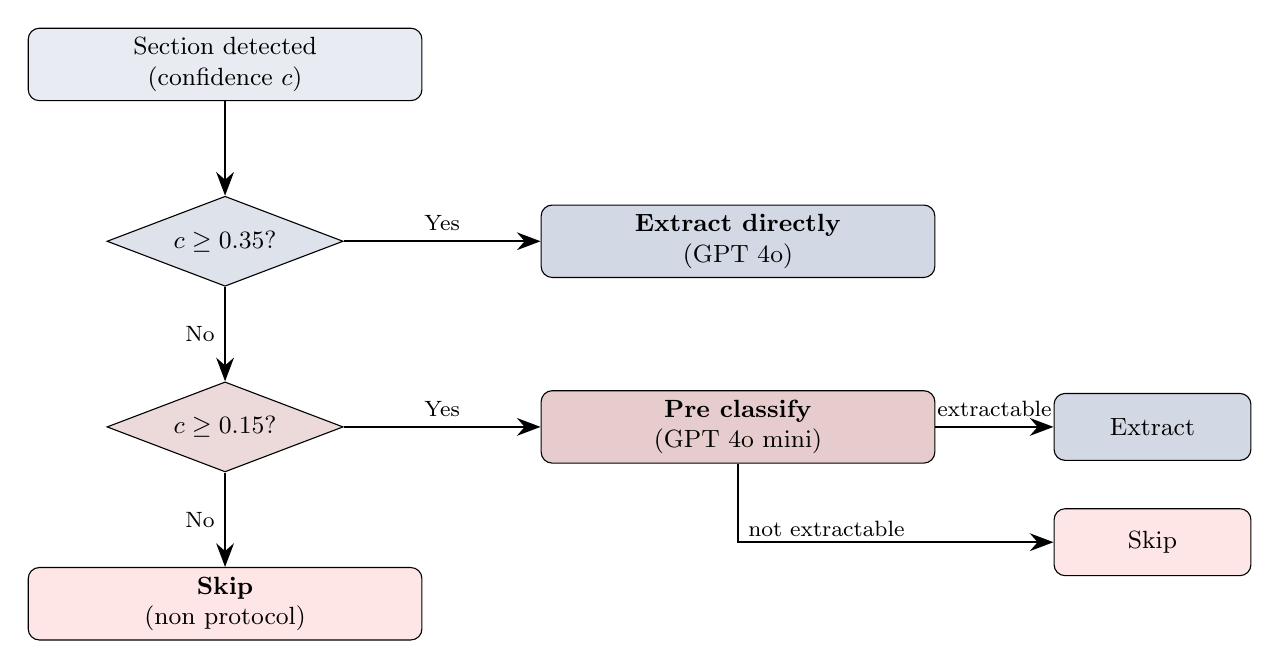
\begin{tikzpicture}[
    node distance=1.2cm,
    box/.style={draw, rounded corners, minimum width=5cm,
                minimum height=0.85cm, align=center, font=\small},
    decision/.style={draw, diamond, aspect=2.4, minimum width=3cm,
                     align=center, font=\small},
    arrow/.style={-{Stealth[length=3mm]}, thick},
]
    \node[box, fill=darkblue!10] (detect) {Section detected\\(confidence $c$)};
    \node[decision, below=of detect, fill=darkblue!15] (high) {$c \geq 0.35$?};
    \node[box, right=2.5cm of high, fill=darkblue!20] (extract)
        {\textbf{Extract directly}\\(GPT 4o)};
    \node[decision, below=of high, fill=deepred!15] (mid) {$c \geq 0.15$?};
    \node[box, right=2.5cm of mid, fill=deepred!20] (classify)
        {\textbf{Pre classify}\\(GPT 4o mini)};
    \node[box, below=of mid, fill=lightpink] (skip) {\textbf{Skip}\\(non protocol)};

    \draw[arrow] (detect) -- (high);
    \draw[arrow] (high) -- node[above, font=\footnotesize]{Yes} (extract);
    \draw[arrow] (high) -- node[left, font=\footnotesize]{No} (mid);
    \draw[arrow] (mid) -- node[above, font=\footnotesize]{Yes} (classify);
    \draw[arrow] (mid) -- node[left, font=\footnotesize]{No} (skip);

    \node[box, right=1.5cm of classify, fill=darkblue!20,
          minimum width=2.5cm] (promote) {Extract};
    \node[box, below=0.6cm of promote, fill=lightpink,
          minimum width=2.5cm] (drop) {Skip};
    \draw[arrow] (classify) -- node[above, font=\footnotesize]
        {extractable} (promote);
    \draw[arrow] (classify) |- node[below right, font=\footnotesize, pos=0.3]
        {not extractable} (drop);
\end{tikzpicture}
\caption{Three tier confidence gate. The middle band uses a cheap
classifier so that borderline sections are not silently dropped.}
\label{fig:gating}
\end{figure}

The middle band exists because a strict threshold either lets in too
many non protocol sections or excludes legitimate protocols whose
formatting deviates from the heuristics. A lightweight call to GPT 4o
mini, which costs roughly one tenth of a GPT 4o call, examines the
first 1500 characters of the section and decides whether to promote it
to full extraction. On IRPG 2025 this band promotes seven sections
that the threshold alone would have skipped, including Burn Injuries
and Heat Related Injury.

\subsection{Stage 4. LLM Extraction}

The fourth stage is the primary LLM call. For each section that
survives the gate, the extractor builds a prompt and asks GPT 4o for a
JSON document that conforms to the protocol graph schema. The prompt
has four ingredients.

\subsubsection{Twenty One Rule System Prompt}

The system prompt contains 21 numbered rules organised into four
categories. Table~\ref{tab:prompt-rules} summarises the categories.
The rules are explicit because the model otherwise tends to merge
branching protocols into linear paths or invent intermediate steps.

\begin{table}[H]
\centering
\begin{tabularx}{\textwidth}{l c X}
\toprule
\textbf{Category} & \textbf{Rules} & \textbf{Focus} \\
\midrule
Structure          & 1 to 4   & One start node, sequential ids, no orphan nodes, evidence required. \\
Node Types         & 5 to 7   & Action, decision, start, end and protocol type classification. \\
Edge and Branching & 8 to 14  & Decision nodes need two or more outgoing edges with different conditions, explicit if then else modelling, branch reconnection, source order preservation, descriptive condition labels. \\
Anti Over Extraction & 15 to 18 & Distinguish sequential from hierarchical, no invented steps, prefer fewer granular nodes, observation versus decision distinction. \\
Metadata           & 19 to 21 & Cross references, confidence scoring, JSON only output. \\
\bottomrule
\end{tabularx}
\caption{Categories of the 21 rule system prompt used during extraction.}
\label{tab:prompt-rules}
\end{table}

\subsubsection{Three Few Shot Examples}

Three manually annotated protocols are appended to the prompt as
examples. CPR demonstrates a moderately branching decision tree, Burn
Injuries demonstrates a linear sequential protocol and Multi Casualty
Triage demonstrates a complex multi branch decision tree with five
decision nodes. Together the three examples cover the main shapes the
model must produce.

\subsubsection{TOC Context}

The detector knows where each section sits in the document hierarchy.
That information is forwarded to the prompt as a category breadcrumb,
for example \texttt{Emergency Medical Care~$\rightarrow$~CPR}, and as
a list of up to ten sibling section titles. The breadcrumb anchors
the model in the document, and the sibling list helps it scope cross
references and avoid pulling content from neighbouring sections.

\subsubsection{Image and Mermaid Input for Diagrams}

Sections whose format hint is \texttt{decision\_tree} or
\texttt{hybrid} are extracted with both their text and a rendering of
the page image. Before being fed to the main extractor, the page image
is converted into a Mermaid diagram by a dedicated GPT 4o call. The
pipeline follows the \emph{TextFlow} intermediate representation
approach (Ye et al. 2024): rather than asking a single multimodal call
to produce the protocol graph from raw pixels, the image is first
turned into a structured text artefact and only then handed to the
extractor. The Mermaid text is injected into the prompt under the
heading \texttt{FLOWCHART~STRUCTURE} together with the instruction
that it is more reliable than the raw text for arrow directions.

\subsection{Stage 5. Edge Review}

The first thing that goes wrong with extracted graphs is almost always
edges. Either the model misses a branch, or it labels both branches of
a decision node with the same condition, or it forgets to reconnect
two branches into a shared downstream step. The edge review stage is a
focused second pass that addresses only edges. It is implemented as a
GPT 4o mini call that receives the extracted graph and the source text
and is asked six specific questions.

\begin{enumerate}[leftmargin=2em]
    \item Does every decision node have two or more outgoing edges
    with different conditions?
    \item Do all branches reconnect to a shared downstream step or to
    an end node?
    \item Are sequential action steps connected in source order?
    \item Are there any fabricated edges that do not correspond to
    source text?
    \item Are there any duplicate edges?
    \item Are there any dangling branches that never reach an end?
\end{enumerate}

A safeguard ensures that a corrected graph is only accepted if it
reduces the total number of structural issues. This guarantees that
the reviewer can never make extraction worse. Because GPT 4o mini is
about ten times cheaper than GPT 4o, the review adds only a modest
overhead per protocol.

\subsection{Stage 6. Validation}

The validation stage applies two layers of checks to every extracted
graph. The structural layer is deterministic and runs without an LLM.
The semantic layer asks GPT 4o to compare the graph against the source
text and surface any remaining issues.

\subsubsection{Structural Checks}

The structural validator implements eight rules.

\begin{enumerate}[leftmargin=2em]
    \item Exactly one start node exists.
    \item At least one end node exists.
    \item Every edge endpoint refers to an existing node id.
    \item No node is orphaned.
    \item Every decision node has at least two outgoing edges.
    \item Every outgoing edge of a decision node carries a condition
    label.
    \item Start nodes have no incoming edges.
    \item End nodes have no outgoing edges.
\end{enumerate}

Two warning level checks flag non sequential node ids and duplicate
edges but do not mark the graph invalid.

\subsubsection{Semantic Review}

The semantic validator examines eight aspects of the graph against the
section text, summarised in Table~\ref{tab:semantic}. When issues are
found the validator may return a corrected graph. As with the edge
reviewer, a guard ensures the corrected graph cannot increase the
number of structural errors.

\begin{table}[H]
\centering
\begin{tabularx}{\textwidth}{l X}
\toprule
\textbf{Aspect} & \textbf{Question} \\
\midrule
Completeness    & Are any steps from the source text missing? \\
Accuracy        & Are any fabricated steps present? \\
Ordering        & Are the steps in source order? \\
Branching       & Are the decision branches and their conditions correct? \\
Granularity     & Are nodes at an appropriate level of detail? \\
Node types      & Are the type assignments correct? \\
Edge conditions & Are the condition labels accurate and complete? \\
Structure       & Does the graph follow the schema rules? \\
\bottomrule
\end{tabularx}
\caption{The eight aspects checked by the semantic validator.}
\label{tab:semantic}
\end{table}

\subsection{Stage 7. Output}

The final stage writes one JSON file per protocol into
\texttt{evaluation/extracted/} and updates a manifest that lists every
extracted protocol with its node and edge counts, source pages and
validation status. The manifest is what drives the interactive viewer
described later in this document.

A separate utility loads the JSON files into a Neo4j database. Neo4j
is not part of the extraction pipeline itself. It is a downstream
storage and query layer that exists because once protocols are
expressed as graphs, the questions worth asking are graph queries.
Examples include locating every protocol that depends on a piece of
equipment or finding all decision points that branch on a particular
condition. JSON files alone cannot answer these questions without ad
hoc traversal code.

\subsection{Why These Decisions}

The architecture is the result of several choices that are worth
making explicit, because each choice trades something against
something else.

\begin{conceptbox}
\textbf{Why an LLM and not a rule based parser.}\\
Emergency protocols are written in natural language and use vocabulary
specific to the domain. A rule based parser would need a separate set
of patterns for each document. A general purpose LLM with a tight
prompt and few shot examples generalises across documents and across
formats without a per document engineering effort. The price is non
determinism, which the validation stage is designed to mitigate.
\end{conceptbox}

\begin{conceptbox}
\textbf{Why TOC first, heuristic second.}\\
Using the TOC as the primary signal gives the detector a high
precision starting point, because TOC entries are explicit
declarations by the document author. Heuristic detection is reserved
as a fallback for documents without a usable TOC. This avoids the
classifier becoming a research problem in itself.
\end{conceptbox}

\begin{conceptbox}
\textbf{Why a confidence gate with three tiers.}\\
A two way threshold either admits too many non protocol sections or
silently rejects legitimate protocols whose markers are weak. The
middle tier uses a cheap classifier to resolve those borderline cases
without paying the cost of the main extractor. On IRPG 2025 this band
recovers seven protocols that a binary threshold would have dropped.
\end{conceptbox}

\begin{conceptbox}
\textbf{Why GPT 4o for extraction and GPT 4o mini for review.}\\
The main extraction call needs the strongest available model because
it has to reason about the structure of the protocol from scratch.
Edge review and pre classification are narrower tasks where GPT 4o
mini is sufficient and roughly ten times cheaper. Splitting the work
this way keeps the pipeline affordable per protocol.
\end{conceptbox}

\begin{conceptbox}
\textbf{Why two loaders for PDFs.}\\
PyMuPDF is fast and faithful for free flowing text but flattens
tables. Docling preserves table structure but is slower and heavier.
Routing sections by their format hint pays the Docling cost only
where it matters and falls back to PyMuPDF if Docling is not
installed. This keeps Docling a soft dependency rather than a hard
one.
\end{conceptbox}

\begin{conceptbox}
\textbf{Why image to Mermaid for diagrams.}\\
A multimodal LLM call that takes a page image as input often produces
graphs in which arrow direction or branch reconnection is wrong.
Producing an explicit Mermaid representation first turns the visual
into text the extractor can read precisely. This is the
\emph{TextFlow} intermediate representation approach (Ye et al.
2024): image $\rightarrow$ structured text $\rightarrow$ downstream
extraction. The Mermaid step exists purely to make the second call
more reliable.
\end{conceptbox}

\begin{conceptbox}
\textbf{Why two stages of validation.}\\
The structural stage catches schema violations cheaply and
deterministically. The semantic stage catches issues that require
reading the source text. Doing structural validation first means the
semantic call only ever sees graphs that are at least well formed,
which makes its job narrower and its outputs more trustworthy. A
guard refuses any correction that introduces new structural errors,
so neither stage can make a graph worse.
\end{conceptbox}

\begin{conceptbox}
\textbf{Why JSON files first and Neo4j second.}\\
Persistence as JSON keeps the pipeline self contained. A graph
database is only required once cross protocol queries become
interesting. Decoupling storage from extraction means the pipeline
can run end to end without Neo4j installed and that the JSON files
remain the canonical source of truth.
\end{conceptbox}

\subsection{Empirical Results}
\label{sec:results}

The pipeline is evaluated against three reference points: the five
hand annotated IRPG protocols, the PET dataset (Neuberger et al.
2024) and the BREX dataset (Yang et al. 2025). The PET and BREX
results are taken directly from
\texttt{evaluation/pet\_benchmark\_results.json} and
\texttt{evaluation/brex\_benchmark\_results.json}.

\subsubsection{IRPG Gold Standard Protocols}

The five IRPG protocols are evaluated by \texttt{eval\_batch.py}
against the gold annotations stored in \texttt{evaluation/gold/}.
Table~\ref{tab:gold-sizes} lists the annotated graph sizes.

\begin{table}[H]
\centering
\begin{tabularx}{\textwidth}{X c c c}
\toprule
\textbf{Protocol} & \textbf{Nodes} & \textbf{Edges} & \textbf{Decision points} \\
\midrule
Burn Injuries        & 14 & 14 & 1 \\
CPR                  & 17 & 19 & 4 \\
Patient Assessment   & 20 & 21 & 3 \\
Risk Management      & 14 & 17 & 3 \\
Multi Casualty Triage & 15 & 20 & 5 \\
\bottomrule
\end{tabularx}
\caption{Gold standard annotation sizes for the five IRPG protocols
used as the quantitative evaluation set.}
\label{tab:gold-sizes}
\end{table}

The pipeline reached its current quality through four incremental
stages of work. Figure~\ref{fig:irpg-progression} traces the average
Node F1 and Edge F1 across those stages on the same five gold
protocols. Edge F1 is the metric that moved most dramatically: the
edge prompt and edge review pass alone lifted it from 0.43 to 0.69,
the single largest jump in the pipeline's history, and the anti over
extraction round closed the remaining gap. By the final round the
two metrics meet at the same level, which is the signal the pipeline
is no longer mis-shaping graphs at the edge level.

\begin{figure}[H]
\centering
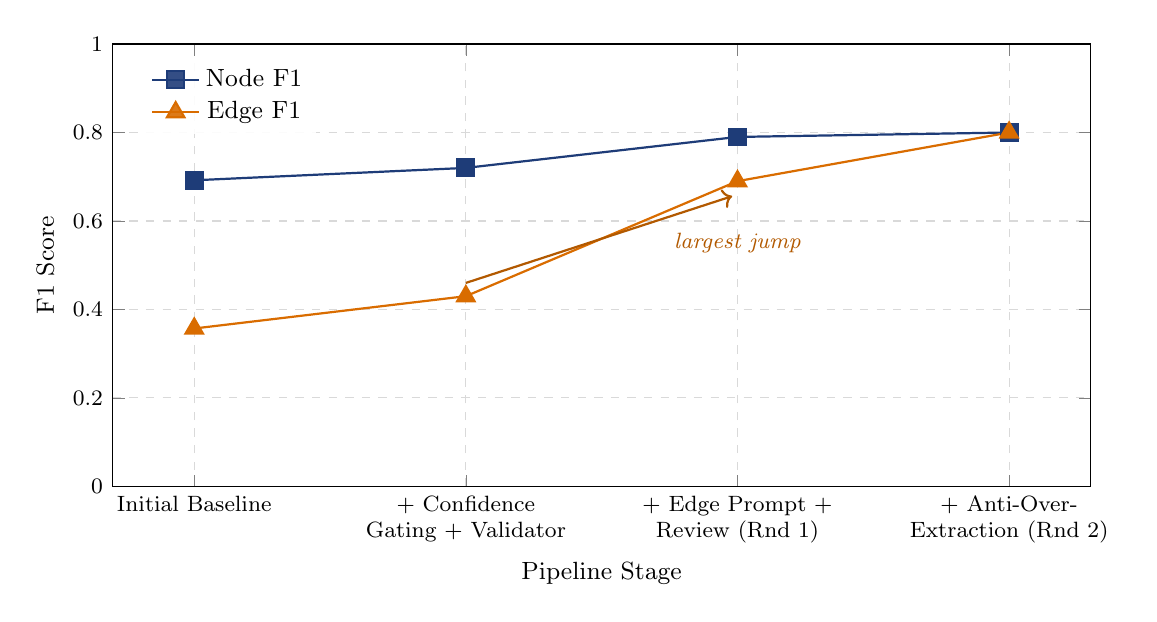
\begin{tikzpicture}
\begin{axis}[
    width=14cm, height=7.2cm,
    xlabel={Pipeline Stage},
    ylabel={F1 Score},
    ymin=0, ymax=1,
    xtick=data,
    symbolic x coords={Initial Baseline,
                       {+ Confidence Gating + Validator},
                       {+ Edge Prompt + Review (Rnd 1)},
                       {+ Anti-Over-Extraction (Rnd 2)}},
    xticklabel style={align=center, font=\footnotesize, text width=2.8cm},
    legend pos=north west,
    legend style={font=\small, draw=none, fill=white, fill opacity=0.9,
                  text opacity=1},
    grid=major,
    grid style={dashed, gray!30},
    label style={font=\small},
    tick label style={font=\footnotesize},
    every axis plot/.append style={thick, mark size=3pt},
]
\addplot[color=darkblue, mark=square*, mark options={fill=darkblue}]
    coordinates {
        (Initial Baseline, 0.692)
        ({+ Confidence Gating + Validator}, 0.72)
        ({+ Edge Prompt + Review (Rnd 1)}, 0.79)
        ({+ Anti-Over-Extraction (Rnd 2)}, 0.80)
    };
\addplot[color=orange!85!black, mark=triangle*,
         mark options={fill=orange!85!black, scale=1.2}]
    coordinates {
        (Initial Baseline, 0.357)
        ({+ Confidence Gating + Validator}, 0.43)
        ({+ Edge Prompt + Review (Rnd 1)}, 0.69)
        ({+ Anti-Over-Extraction (Rnd 2)}, 0.80)
    };
\legend{Node F1, Edge F1}
\node[font=\footnotesize\itshape, color=orange!70!black]
    at (axis cs:{+ Edge Prompt + Review (Rnd 1)}, 0.55) {largest jump};
\draw[->, thick, orange!70!black, shorten >=2pt]
    (axis cs:{+ Confidence Gating + Validator}, 0.46)
    -- (axis cs:{+ Edge Prompt + Review (Rnd 1)}, 0.66);
\end{axis}
\end{tikzpicture}
\caption{Average Node F1 and Edge F1 on the five IRPG gold standard
protocols across the four iterations of the pipeline. The
\emph{Initial Baseline} stage uses the figures hardcoded in
\texttt{eval\_batch.py} (Node F1 0.69, Edge F1 0.36). Edge F1
gains the most from adding the edge prompt and the GPT 4o mini edge
review pass, which the arrow highlights as the single largest jump.
The final round of anti over extraction rules closes the remaining
gap and brings the two metrics together.}
\label{fig:irpg-progression}
\end{figure}

\subsubsection{PET Cross Domain Benchmark}

The PET benchmark (\texttt{evaluation/pet\_benchmark.py}) runs the
pipeline on ten PET documents and compares Activity F1 against the
gold action node spans and Edge F1 against the gold sequence flows.
Figure~\ref{fig:pet-results} compares the run to the published
baselines. The pipeline reports zero extraction errors on PET.

\begin{figure}[H]
\centering
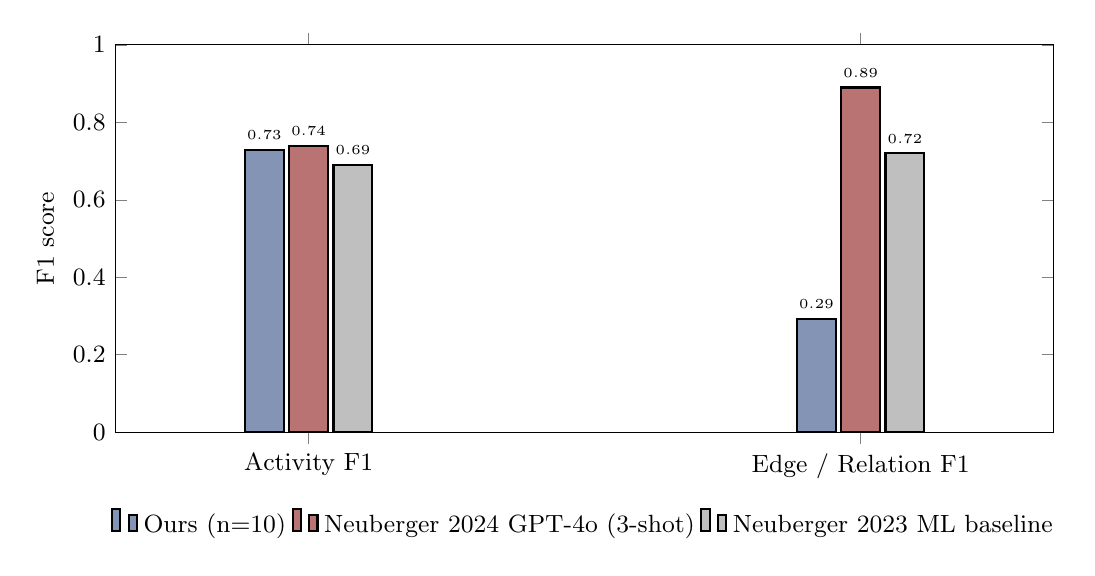
\begin{tikzpicture}
\begin{axis}[
    ybar,
    bar width=14pt,
    width=13.5cm, height=6.5cm,
    enlarge x limits=0.35,
    ymin=0, ymax=1,
    ylabel={F1 score},
    symbolic x coords={Activity F1, Edge / Relation F1},
    xtick=data,
    nodes near coords,
    nodes near coords style={font=\tiny,
        /pgf/number format/.cd, fixed, zerofill, precision=2},
    legend style={at={(0.5,-0.18)}, anchor=north, legend columns=3,
                  font=\small, draw=none},
    every axis plot/.append style={draw=black, thick},
    tick label style={font=\small},
    label style={font=\small},
]
\addplot[fill=darkblue!55] coordinates {
    (Activity F1, 0.728)
    (Edge / Relation F1, 0.293)
};
\addplot[fill=deepred!55] coordinates {
    (Activity F1, 0.74)
    (Edge / Relation F1, 0.89)
};
\addplot[fill=gray!50] coordinates {
    (Activity F1, 0.69)
    (Edge / Relation F1, 0.72)
};
\legend{Ours (n=10), Neuberger 2024 GPT-4o (3-shot), Neuberger 2023 ML baseline}
\end{axis}
\end{tikzpicture}
\caption{PET benchmark. Activity F1 measures action node extraction
and is on par with the published GPT 4o three shot baseline. Edge
F1 trails the published Relation F1 because PET edges are
token level relation spans whereas the pipeline produces graph
edges between summarised action nodes; the two are not strictly
like for like and the gap is the expected mismatch flagged in the
benchmark docstring. Branching accuracy on the same run is 0.75
and node type accuracy is 0.76.}
\label{fig:pet-results}
\end{figure}

\subsubsection{BREX Cross Lingual Benchmark}

The BREX benchmark (\texttt{evaluation/brex\_benchmark.py}) runs the
pipeline on Chinese business rules using the English system prompt.
Figure~\ref{fig:brex-results} compares the run to the four published
baselines from Yang et al. 2025. The recorded run completed two
documents successfully and lost the remaining eight to upstream
connection errors, so the bar marked \emph{Ours} is reported with
$n = 2$ and should be read as a directional signal rather than a
confident estimate.

\begin{figure}[H]
\centering
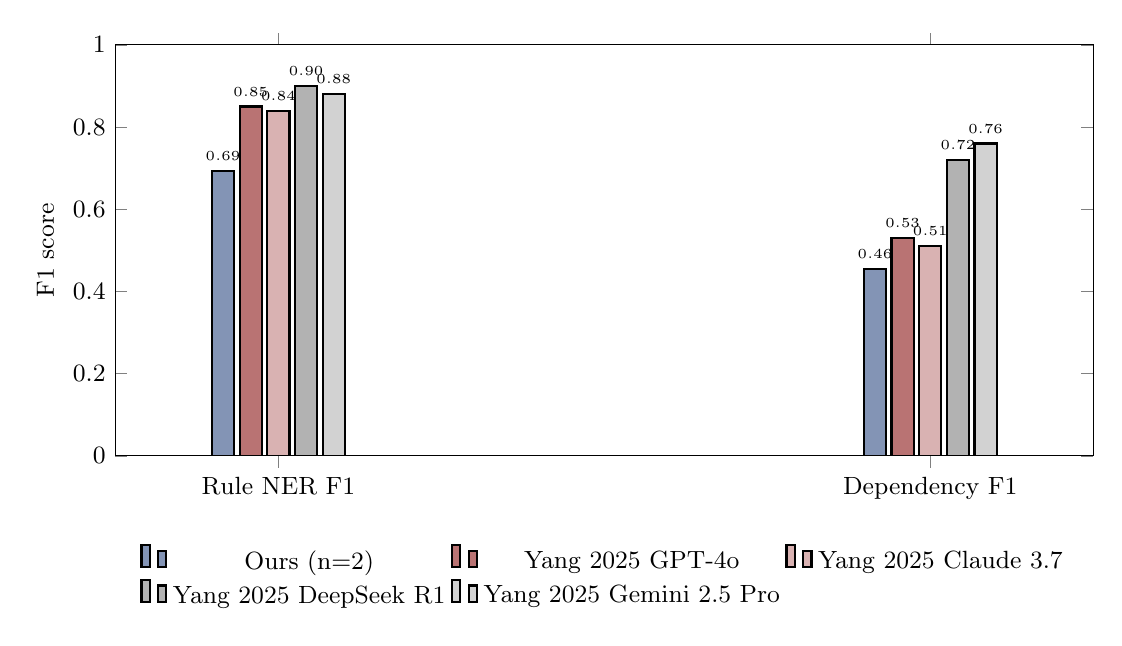
\begin{tikzpicture}
\begin{axis}[
    ybar,
    bar width=8pt,
    width=14cm, height=6.8cm,
    enlarge x limits=0.25,
    ymin=0, ymax=1,
    ylabel={F1 score},
    symbolic x coords={Rule NER F1, Dependency F1},
    xtick=data,
    nodes near coords,
    nodes near coords style={font=\tiny,
        /pgf/number format/.cd, fixed, zerofill, precision=2},
    legend style={at={(0.5,-0.20)}, anchor=north, legend columns=3,
                  font=\small, draw=none},
    every axis plot/.append style={draw=black, thick},
    tick label style={font=\small},
    label style={font=\small},
]
\addplot[fill=darkblue!55] coordinates {
    (Rule NER F1, 0.694)
    (Dependency F1, 0.455)
};
\addplot[fill=deepred!55] coordinates {
    (Rule NER F1, 0.85)
    (Dependency F1, 0.53)
};
\addplot[fill=deepred!30] coordinates {
    (Rule NER F1, 0.84)
    (Dependency F1, 0.51)
};
\addplot[fill=gray!60] coordinates {
    (Rule NER F1, 0.90)
    (Dependency F1, 0.72)
};
\addplot[fill=gray!35] coordinates {
    (Rule NER F1, 0.88)
    (Dependency F1, 0.76)
};
\legend{Ours (n=2), Yang 2025 GPT-4o, Yang 2025 Claude 3.7,
        Yang 2025 DeepSeek R1, Yang 2025 Gemini 2.5 Pro}
\end{axis}
\end{tikzpicture}
\caption{BREX benchmark. Rule NER F1 corresponds to node matching
and Dependency F1 to edge matching. The pipeline trails the GPT 4o
baseline on Rule NER and lands between Claude 3.7 and Gemini 2.5
Pro on Dependency F1, on a sample of two. The eight connection
errors in the recorded run are kept in the JSON results file so
they remain visible.}
\label{fig:brex-results}
\end{figure}

\subsection{What Each Component Owns}

Table~\ref{tab:components} gives a one line summary of every module in
the pipeline. The detailed code documentation follows in the next
pass.

\begin{table}[H]
\centering
\small
\begin{tabularx}{\textwidth}{l l X}
\toprule
\textbf{Layer} & \textbf{Module} & \textbf{Responsibility} \\
\midrule
Ingestion  & \texttt{pdf\_ingest.py}        & PyMuPDF based text, table, TOC and image extraction. \\
Ingestion  & \texttt{docling\_loader.py}    & Optional Docling parser for table heavy sections. \\
\addlinespace
Extraction & \texttt{section\_detector.py}  & TOC and heuristic protocol section detection with confidence scoring. \\
Extraction & \texttt{batch\_extractor.py}   & Pipeline orchestrator that wires the gate, the extractor, the reviewer and the validator. \\
Extraction & \texttt{protocol\_extractor.py}& LLM extraction with system prompt, few shot examples, multimodal support and edge review. \\
Extraction & \texttt{validator.py}          & Two stage structural and semantic validator with auto correction safeguard. \\
\addlinespace
Graph      & \texttt{neo4j\_export.py}      & Loads extracted JSON graphs into Neo4j. \\
Graph      & \texttt{kg\_enrichment.py}     & Optional second pass that annotates protocols with semantic entities. \\
Graph      & \texttt{pet\_adapter.py}       & PET dataset adapter for cross domain evaluation. \\
Graph      & \texttt{brex\_adapter.py}      & BREX dataset adapter for cross lingual evaluation. \\
\addlinespace
Top level  & \texttt{run\_full\_batch.py}   & Main entry point that runs the pipeline on a PDF. \\
Top level  & \texttt{evaluate.py}           & Node and edge precision, recall and F1 metrics. \\
Top level  & \texttt{eval\_batch.py}        & Compares batch output against gold standards. \\
Top level  & \texttt{generate\_manifest.py} & Builds the manifest that the viewer reads. \\
Top level  & \texttt{load\_neo4j.py}        & Loads all extracted graphs into Neo4j. \\
Top level  & \texttt{visualize.py}          & Produces side by side PNG comparisons of graphs. \\
\addlinespace
Benchmarks & \texttt{evaluation/parser\_benchmark.py} & Compares PyMuPDF and Docling on the same pages. \\
Benchmarks & \texttt{evaluation/pet\_benchmark.py}    & Runs the pipeline on PET and reports metrics. \\
Benchmarks & \texttt{evaluation/brex\_benchmark.py}   & Runs the pipeline on BREX and reports metrics. \\
\addlinespace
Artifacts  & \texttt{schema/protocol\_schema.json} & The JSON Schema for protocol graphs. \\
Artifacts  & \texttt{viewer.html}                  & Interactive web viewer for extracted protocols. \\
Artifacts  & \texttt{docker-compose.yml}           & Neo4j 5 Community service definition. \\
\bottomrule
\end{tabularx}
\caption{Every module in the pipeline and the one thing it owns.}
\label{tab:components}
\end{table}

% =====================================================================
\section{Code Documentation}
\label{sec:code-doc}

This section documents the source code in the order in which a request
would travel through it. The ingestion layer is described first, then
the extraction layer, then the graph layer, then the entry point
scripts that compose them, then the benchmarks, and finally the
artefacts that surround the code.

For every module the following information is provided. The purpose
sentence states what the module owns. The dependency line lists the
internal modules it imports. The public interface is then enumerated
with brief descriptions, and a note explains how the module is used by
the rest of the system.

\subsection{Project Structure}

\begin{tcolorbox}[colback=mygray, colframe=mygray, sharp corners, boxrule=0pt]
\begin{minted}[fontsize=\footnotesize]{text}
DataPipeline/
+- src/
|  +- ingestion/
|  |  +- pdf_ingest.py        PyMuPDF based loader
|  |  +- docling_loader.py    optional Docling loader
|  +- extraction/
|  |  +- section_detector.py  TOC and heuristic detection
|  |  +- batch_extractor.py   pipeline orchestrator
|  |  +- protocol_extractor.py LLM extraction with edge review
|  |  +- validator.py         structural plus semantic validation
|  +- graph/
|     +- neo4j_export.py      Neo4j writer
|     +- kg_enrichment.py     optional semantic enrichment
|     +- pet_adapter.py       PET to schema mapping
|     +- brex_adapter.py      BREX to schema mapping
+- evaluation/
|  +- gold/                   five gold standard graphs
|  +- extracted/              79 extracted graphs plus manifest
|  +- pet_gold/               PET gold graphs
|  +- parser_benchmark.py     PyMuPDF versus Docling
|  +- pet_benchmark.py        PET cross domain evaluation
|  +- brex_benchmark.py       BREX cross lingual evaluation
+- schema/protocol_schema.json  JSON Schema for protocol graphs
+- run_full_batch.py            primary entry point
+- evaluate.py                  metrics library
+- eval_batch.py                gold standard comparison
+- generate_manifest.py         viewer index generator
+- load_neo4j.py                Neo4j loader CLI
+- visualize.py                 graph rendering utility
+- viewer.html                  interactive web viewer
+- docker-compose.yml           Neo4j 5 Community service
+- IRPG-2025.pdf                source document one
+- VIC-BushfireHandbook.pdf     source document two
\end{minted}
\end{tcolorbox}

% =====================================================================
\subsection{Ingestion Layer}

The ingestion layer turns a PDF on disk into an in memory data
structure that downstream stages can query without ever opening the
file again. There are two loaders. PyMuPDF is the default. Docling is
loaded on demand for table heavy sections.

% ---------------------------------------------------------------------
\subsubsection{src/ingestion/pdf\_ingest.py}

\begin{codeconceptbox}{Purpose}
PyMuPDF based loader that produces the canonical document model. It
reads text blocks with bounding boxes, parses tables when PyMuPDF is
able to detect them, extracts the table of contents and decides
whether the PDF is native or scanned.
\end{codeconceptbox}

\textbf{Internal dependencies.} None.

\textbf{Public types.}

\begin{description}[leftmargin=2em, style=nextline]
\item[\texttt{TextBlock}]
A dataclass with \texttt{text}, \texttt{bbox} as four floats, a
\texttt{block\_type} of \texttt{"text"} or \texttt{"image"} and the
1 based \texttt{page} number.
\item[\texttt{TableData}]
A dataclass holding the table cells as a list of rows, the bounding
box and the page number.
\item[\texttt{PageContent}]
A dataclass that aggregates the text blocks, tables, full text,
dimensions and image flags for a single page.
\item[\texttt{DocumentContent}]
The top level dataclass returned by \texttt{ingest\_pdf}. It carries
the filename, page count, a list of \texttt{PageContent} objects, the
\texttt{toc} as a list of \texttt{\{level, title, page\}} dictionaries
and the \texttt{is\_native} flag.
\end{description}

\textbf{Public functions.}

\begin{description}[leftmargin=2em, style=nextline]
\item[\texttt{ingest\_pdf(pdf\_path)}]
Open the PDF with PyMuPDF, walk every page, build a
\texttt{PageContent} per page, read the TOC and return a fully
populated \texttt{DocumentContent}. The native flag is set when more
than half of the pages contain extractable text.
\item[\texttt{render\_page\_image(pdf\_path, page\_num, dpi=200)}]
Render a single page to PNG bytes. Used by the multimodal extractor
when a section needs to be sent to the model as an image.
\item[\texttt{save\_document\_json(doc, output\_path)}]
Serialise a \texttt{DocumentContent} to a JSON file. Useful for
caching ingestion results across runs.
\item[\texttt{print\_summary(doc)}]
Print page count, TOC size, table count and sample heading. Used for
manual inspection during development.
\end{description}

\textbf{How the rest of the system uses it.} Every component that
needs to read PDF content imports \texttt{ingest\_pdf} and operates on
the \texttt{DocumentContent} it returns. The section detector, batch
extractor and protocol extractor all consume this same data structure.

% ---------------------------------------------------------------------
\subsubsection{src/ingestion/docling\_loader.py}

\begin{codeconceptbox}{Purpose}
Optional alternative loader that uses IBM Docling to preserve table
structure as Markdown. It is invoked only for sections whose format
hint is \texttt{table}. If Docling is not installed the import fails
silently in the batch extractor and the pipeline falls back to
PyMuPDF.
\end{codeconceptbox}

\textbf{Internal dependencies.} None. Docling itself is imported
lazily inside the public functions.

\textbf{Public functions.}

\begin{description}[leftmargin=2em, style=nextline]
\item[\texttt{extract\_with\_docling(pdf\_path,\allowbreak{} start\_page=None,\allowbreak{} end\_page=None)}]
Convert the PDF to Markdown with Docling and optionally narrow the
output to a page range. The Markdown contains pipe delimited tables
with headers and row separators preserved.
\item[\texttt{extract\_tables\_from\_pages(pdf\_path,\allowbreak{} start\_page,\allowbreak{} end\_page)}]
Iterate over Docling's table items, parse each one into headers and
rows and return a list of \texttt{\{page, headers, rows, markdown\}}
dictionaries. Used when the caller needs structured access to table
content rather than Markdown text.
\end{description}

\textbf{How the rest of the system uses it.} The batch extractor
imports \texttt{extract\_with\_docling} inside a try block. If the
import succeeds it sets a \texttt{HAS\_DOCLING} flag. Sections whose
format hint equals \texttt{"table"} are then routed through Docling
when the flag is on, and through PyMuPDF otherwise.

% =====================================================================
\subsection{Extraction Layer}

The extraction layer is where the work happens. Section detection runs
first to decide which page ranges deserve attention. The batch
extractor then orchestrates the full pipeline. The protocol extractor
performs the LLM call. The validator checks the result.

% ---------------------------------------------------------------------
\subsubsection{src/extraction/section\_detector.py}

\begin{codeconceptbox}{Purpose}
Identify protocol sections within a PDF, classify each one by format
and assign a confidence score that drives the gating stage downstream.
\end{codeconceptbox}

\textbf{Internal dependencies.}
\texttt{src.ingestion.pdf\_ingest} for \texttt{DocumentContent} and
\texttt{PageContent}.

\textbf{Public types.}

\begin{description}[leftmargin=2em, style=nextline]
\item[\texttt{ProtocolSection}]
A dataclass with title, start and end page, TOC level, parent
category, format hint and confidence. It also carries boolean flags
for the markers used to score it: \texttt{has\_tables},
\texttt{has\_numbered\_steps}, \texttt{has\_decision\_logic} and
\texttt{has\_cross\_references}, and an \texttt{is\_protocol} flag
that the detector sets to false for known non protocol sections such
as glossaries, indices and appendices.
\item[\texttt{DetectionResult}]
The container returned by \texttt{detect\_sections}. It carries the
list of \texttt{ProtocolSection}, the unique categories, the total
count of protocol sections and the detection method
(\texttt{"toc"}, \texttt{"heuristic"} or \texttt{"hybrid"}).
\end{description}

\textbf{Public functions.}

\begin{description}[leftmargin=2em, style=nextline]
\item[\texttt{detect\_sections(doc)}]
Main entry point. If the document carries a TOC, walk it and treat
every entry as a section. Otherwise fall back to heuristic detection.
For every section, classify the format and compute the confidence.
\item[\texttt{print\_detection\_summary(result)}]
Pretty print categories, sections and per format counts for manual
inspection.
\end{description}

\textbf{Confidence formula in code.} The score adds 0.25 for a
protocol keyword in the title, 0.20 each for numbered steps and
decision logic, 0.10 for tables, 0.15 for sections of one to ten
pages (0.05 for longer sections) and 0.10 for imperative action
language, capped at 1.0. The flag thresholds are at least two
numbered step matches, at least one decision pattern match and at
least one imperative match (three are required to trigger the
\texttt{checklist} format). Sections matching the
\texttt{NON\_PROTOCOL\_TITLES} regular expression have
\texttt{is\_protocol} set to false and are forced to confidence
zero. The full breakdown, including the format hint cascade and the
non protocol title list, is in
Section~\ref{sec:architecture}.

\textbf{How the rest of the system uses it.} The batch extractor calls
\texttt{detect\_sections} once per PDF. The resulting list drives both
the gating stage and the TOC context that is appended to every
extraction prompt.

% ---------------------------------------------------------------------
\subsubsection{src/extraction/batch\_extractor.py}

\begin{codeconceptbox}{Purpose}
Pipeline orchestrator. It wires the section detector, the confidence
gate, the pre classifier, the extractor, the edge reviewer and the
validator together. It is the single function that
\texttt{run\_full\_batch.py} calls.
\end{codeconceptbox}

\textbf{Internal dependencies.}
\begin{itemize}[leftmargin=2em, nosep, label={--}]
\item \texttt{src.ingestion.pdf\_ingest}
\item \texttt{src.ingestion.docling\_loader} (optional)
\item \texttt{src.extraction.section\_detector}
\item \texttt{src.extraction.protocol\_extractor}
\item \texttt{src.extraction.validator}
\end{itemize}

\textbf{Public types.}

\begin{description}[leftmargin=2em, style=nextline]
\item[\texttt{BatchConfig}]
Dataclass holding every knob the pipeline exposes. Notable fields are
\texttt{extract\_threshold} (default 0.35),
\texttt{classify\_threshold} (default 0.15),
\texttt{use\_multimodal} (off by default),
\texttt{multimodal\_formats} which controls which format hints
trigger image input,
\texttt{use\_few\_shot} (default true),
\texttt{use\_edge\_review} (default true) with
\texttt{edge\_review\_model} set to \texttt{"gpt-4o-mini"},
\texttt{use\_docling\_for\_tables} (default true),
\texttt{use\_validator} (off by default),
\texttt{validator\_model} set to \texttt{"gpt-4o"},
\texttt{model} set to \texttt{"gpt-4o"} and
\texttt{output\_dir} defaulting to
\texttt{"evaluation/extracted"}. A \texttt{dry\_run} flag prints the
plan without calling the API.
\item[\texttt{ExtractionResult}]
The outcome of a single section. Carries the section, a status string,
the extracted graph, an error message, the token count, the elapsed
time and an optional \texttt{ValidationResult}.
\item[\texttt{BatchResult}]
The outcome of a full document run. Aggregates per status counts,
total tokens and total time alongside the per section
\texttt{ExtractionResult} list.
\end{description}

\textbf{Public functions.}

\begin{description}[leftmargin=2em, style=nextline]
\item[\texttt{pre\_classify\_section}]
Full call:
\texttt{pre\_classify\_section(section,\allowbreak{} doc,\allowbreak{}
client,\allowbreak{} model="gpt-4o-mini")}.
Send the first 1500 characters of a borderline section to GPT 4o mini
with the \texttt{PRE\_CLASSIFY\_PROMPT} and parse the
\texttt{is\_extractable} field from the JSON response.
\item[\texttt{build\_toc\_context(section, detection)}]
Build the breadcrumb and sibling list that is injected into the
extraction prompt. Sibling titles are capped at ten.
\item[\texttt{plan\_batch(detection, config)}]
Partition the detected sections into three lists.
\texttt{to\_extract} contains sections whose confidence is at or
above the extract threshold. \texttt{to\_classify} contains sections
in the middle band. \texttt{to\_skip} contains the rest.
\item[\texttt{run\_batch(pdf\_path, config=None)}]
The full pipeline. Ingest, detect, partition, pre classify the
borderline list, extract every section that survives, route table
sections through Docling when enabled, run the edge reviewer when
enabled, run the two stage validator when enabled and persist every
graph as JSON in the output directory.
\end{description}

\textbf{How the rest of the system uses it.} \texttt{run\_full\_batch.py}
constructs a \texttt{BatchConfig}, calls \texttt{run\_batch} for each
target PDF and prints the resulting summary.

% ---------------------------------------------------------------------
\subsubsection{src/extraction/protocol\_extractor.py}

\begin{codeconceptbox}{Purpose}
Owns every interaction with the OpenAI Chat Completions API. Holds the
21 rule \texttt{SYSTEM\_PROMPT}, the table specific
\texttt{TABLE\_EXTRACTION\_PROMPT}, the few shot example loader, the
multimodal extractor with its image to Mermaid intermediate
representation and the edge review pass.
\end{codeconceptbox}

\textbf{Internal dependencies.}
\begin{itemize}[leftmargin=2em, nosep, label={--}]
\item \texttt{src.ingestion.pdf\_ingest}
  (for \texttt{DocumentContent} and \texttt{render\_page\_image})
\item \texttt{src.extraction.section\_detector}
  (for \texttt{ProtocolSection})
\end{itemize}

\textbf{Public functions.}

\begin{description}[leftmargin=2em, style=nextline]
\item[\texttt{extract\_protocol}]
Full call:
\texttt{extract\_protocol(section,\allowbreak{} doc,\allowbreak{}
model="gpt-4o",\allowbreak{} use\_few\_shot=True,\allowbreak{}
toc\_context=None)}.
Build the prompt with the system instructions, the few shot
exchanges, the TOC context, the format hint and the section text.
Send to GPT 4o with temperature 0.1 and JSON object response format.
Return the parsed graph with attached
\texttt{\_extraction\_meta}.
\item[\texttt{extract\_protocol\_from\_text}]
Full call:
\texttt{extract\_protocol\_from\_text(title,\allowbreak{}
section\_text,\allowbreak{} pages,\allowbreak{} source\_pdf,\allowbreak{}
format\_hint="unknown",\allowbreak{} model="gpt-4o",\allowbreak{}
use\_few\_shot=True)}.
Variant that operates on raw text rather than a
\texttt{ProtocolSection}. Used by the PET and BREX benchmarks where
no real PDF section exists.
\item[\texttt{extract\_protocol\_multimodal}]
Full call:
\texttt{extract\_protocol\_multimodal(section,\allowbreak{}
doc,\allowbreak{} pdf\_path,\allowbreak{} model="gpt-4o",\allowbreak{}
use\_few\_shot=True,\allowbreak{} dpi=200,\allowbreak{}
toc\_context=None)}.
Render every page in the section, encode them as base64 PNG and pass
both text and images to the model. For \texttt{decision\_tree} and
\texttt{hybrid} formats, run \texttt{\_image\_to\_mermaid} first and
inject the resulting Mermaid block into the prompt under the heading
\texttt{FLOWCHART STRUCTURE}.
\item[\texttt{review\_edges(extracted,\allowbreak{} source\_text,\allowbreak{} model="gpt-4o-mini")}]
Send the graph and source text to GPT 4o mini with the
\texttt{EDGE\_REVIEW\_PROMPT} and replace the graph if the reviewed
version reports fewer issues. The check uses
\texttt{\_count\_edge\_issues} so the reviewer can never make the
graph worse. If the response is empty or unparseable the original
graph is returned unchanged.
\item[\texttt{save\_extraction(graph, path)}]
Write the graph to a JSON file with indentation.
\end{description}

\textbf{Two system prompts.} The default \texttt{SYSTEM\_PROMPT}
contains the 21 rules summarised in Table~\ref{tab:prompt-rules}. A
shorter \texttt{TABLE\_EXTRACTION\_PROMPT} is selected automatically
when the section's \texttt{format\_hint} equals \texttt{"table"}.
The table prompt instructs the model to model each row as a
condition $\rightarrow$ action pair when both columns are present,
as a sequential checklist when only an action column is present and
to use any grouping or severity column as decision branches. It
asks the model to preserve cell text verbatim rather than
paraphrase, and repeats a compact subset of the structural rules
(single start, decision branching, sequential ids, evidence per
node).

\textbf{Internal helpers worth knowing about.}

\begin{description}[leftmargin=2em, style=nextline]
\item[\texttt{\_safe\_json\_loads(raw)}]
Parses LLM output that may be wrapped in Markdown code fences, may
contain invalid \texttt{\textbackslash uXXXX} sequences or may include
trailing prose. Falls back to extracting the first
\texttt{\{...\}} block if the body is not valid JSON.
\item[\texttt{\_load\_few\_shot\_examples()}]
Reads the three gold standard files \texttt{cpr\_01.json},
\texttt{burn\_injuries\_01.json} and \texttt{triage\_01.json} from
\texttt{evaluation/gold}.
\item[\texttt{\_build\_few\_shot\_messages(examples)}]
Builds user and assistant message pairs that pair each gold annotation
with the source text it came from.
\item[\texttt{\_image\_to\_mermaid(client, page\_images\_b64, model)}]
Sends page images to GPT 4o with instructions to produce a
\texttt{graph TD} Mermaid diagram. Strips any Markdown fences from the
response.
\item[\texttt{\_count\_edge\_issues(graph)}]
Counts dangling edges, decision nodes with fewer than two outgoing
edges and orphan nodes. Used by the edge review safeguard.
\end{description}

\textbf{How the rest of the system uses it.} The batch extractor
imports \texttt{extract\_protocol},
\texttt{extract\_protocol\_from\_text},
\texttt{extract\_protocol\_multimodal} and \texttt{review\_edges}. The
benchmarks import \texttt{extract\_protocol\_from\_text} and
\texttt{review\_edges}.

% ---------------------------------------------------------------------
\subsubsection{src/extraction/validator.py}

\begin{codeconceptbox}{Purpose}
Apply the eight structural rules deterministically and then ask GPT 4o
to look for semantic issues. Wrap both passes in a single
\texttt{ValidationResult}. Refuse any correction that introduces new
structural errors.
\end{codeconceptbox}

\textbf{Internal dependencies.} None.

\textbf{Public types.}

\begin{description}[leftmargin=2em, style=nextline]
\item[\texttt{StructuralIssue}]
Severity, machine readable code, human readable message and optional
node id.
\item[\texttt{ValidationResult}]
Carries the list of structural issues, the raw semantic result, the
original graph, the corrected graph if any, the
\texttt{was\_corrected} flag, the totals and the validation token
count.
\end{description}

\textbf{Public functions.}

\begin{description}[leftmargin=2em, style=nextline]
\item[\texttt{validate\_structure(graph)}]
Eight checks. One start node, at least one end node, no dangling
edges, no orphan nodes, decision nodes with at least two outgoing
edges, decision edges with conditions, no incoming edges to start
nodes, no outgoing edges from end nodes. Plus warnings for non
sequential ids and duplicate edges.
\item[\texttt{validate\_semantic(graph,\allowbreak{} section\_text,\allowbreak{} model="gpt-4o")}]
Send the graph and source text to GPT 4o with the
\texttt{VALIDATOR\_SYSTEM\_PROMPT}. Returns a dictionary with
\texttt{review\_passed}, \texttt{issues}, \texttt{corrections\_made},
\texttt{correction\_summary} and \texttt{corrected\_graph}.
\item[\texttt{validate\_protocol}]
Full call:
\texttt{validate\_protocol(graph,\allowbreak{} section\_text,\allowbreak{}
run\_semantic=True,\allowbreak{} model="gpt-4o")}.
Run the structural checks first. Run the semantic pass when enabled.
If a corrected graph is returned, accept it only when its structural
issue count is no worse than the original. Return a single
\texttt{ValidationResult}.
\item[\texttt{print\_validation\_summary(result)}]
Pretty print every structural and semantic issue.
\end{description}

\textbf{How the rest of the system uses it.} The batch extractor
calls \texttt{validate\_protocol} for every successful extraction
when \texttt{config.use\_validator} is true. The corrected graph, if
accepted, replaces the extracted graph before it is written to disk.

% =====================================================================
\subsection{Graph Layer}

The graph layer turns extracted protocols into other forms.
\texttt{neo4j\_export.py} loads them into a database.
\texttt{kg\_enrichment.py} annotates them with semantic entities.
The two adapters convert public datasets into the same schema so the
pipeline can be evaluated against them.

% ---------------------------------------------------------------------
\subsubsection{src/graph/neo4j\_export.py}

\begin{codeconceptbox}{Purpose}
Load extracted protocol JSON files into a Neo4j database. Create the
necessary uniqueness constraints, build the labels and relationships
defined by the schema, link cross referenced protocols and provide a
statistics query for inspection.
\end{codeconceptbox}

\textbf{Internal dependencies.} None. Uses the official
\texttt{neo4j} Python driver.

\textbf{Schema produced in Neo4j.}

\begin{description}[leftmargin=2em, style=nextline]
\item[\textbf{Core node labels.}]
\texttt{Protocol} for the top level metadata,
\texttt{Step} for nodes typed start, end or action and
\texttt{Decision} for decision nodes.
\item[\textbf{Entity node labels (when enrichment is present).}]
\texttt{Role}, \texttt{Equipment}, \texttt{Hazard},
\texttt{Condition} and \texttt{IncidentType}. One node is created
per distinct lowercased entity name and shared across every
protocol that mentions it.
\item[\textbf{Core relationship types.}]
\texttt{HAS\_STEP} from a \texttt{Protocol} to each of its
\texttt{Step} or \texttt{Decision} nodes,
\texttt{NEXT} from one \texttt{Step} to the next sequential
\texttt{Step},
\texttt{BRANCHES\_TO} from a \texttt{Decision} to a \texttt{Step}
with the condition stored as a property and
\texttt{CROSS\_REFERENCES} from a \texttt{Protocol} to another
referenced \texttt{Protocol}.
\item[\textbf{Entity relationship types.}]
\texttt{PERFORMED\_BY} to \texttt{Role},
\texttt{REQUIRES} to \texttt{Equipment},
\texttt{INVOLVES\_HAZARD} to \texttt{Hazard},
\texttt{HAS\_CONDITION} to \texttt{Condition} and
\texttt{APPLIES\_TO} to \texttt{IncidentType}. These edges are
emitted both at the \texttt{Protocol} level (for entities listed
in the global \texttt{enrichment.entities} dictionary) and at the
\texttt{Step} or \texttt{Decision} level (for entities listed in
\texttt{enrichment.node\_annotations} for that node).
\end{description}

\textbf{Entity loading is conditional.} The exporter creates entity
nodes and entity relationships only when the protocol JSON contains
an \texttt{enrichment} key. Plain extracted graphs without
enrichment load just the core schema, so running
\texttt{load\_neo4j.py} without \texttt{--enrich} produces a graph
with \texttt{Protocol}, \texttt{Step} and \texttt{Decision} only.

\textbf{Public class.} \texttt{Neo4jExporter} is a context manager.

\begin{description}[leftmargin=2em, style=nextline]
\item[\texttt{\_\_init\_\_(uri, user, password, database="neo4j")}]
Open the Bolt connection with the given credentials.
\item[\texttt{create\_constraints()}]
Create uniqueness constraints on \texttt{Protocol.protocol\_id} and
\texttt{Step.uid} and indexes on \texttt{Step.node\_type} and
\texttt{Step.protocol\_id}.
\item[\texttt{load\_protocol(json\_path)}]
Read a single JSON file and import it. Returns a summary with
\texttt{nodes\_created}, \texttt{edges\_created} and entity counts.
\item[\texttt{load\_all(directory, pattern="*.json")}]
Iterate every JSON file in the directory, skip the manifest and
delegate to \texttt{load\_protocol}.
\item[\texttt{clear\_database()}]
Drop every node and relationship in the configured database.
\item[\texttt{get\_graph\_stats()}]
Return counts of \texttt{Protocol} nodes, \texttt{Step} nodes,
\texttt{Decision} nodes and each relationship type.
\item[\texttt{close()}]
Close the driver. The class also implements \texttt{\_\_enter\_\_}
and \texttt{\_\_exit\_\_} so it can be used in a \texttt{with}
statement.
\end{description}

\textbf{How the rest of the system uses it.}
\texttt{load\_neo4j.py} is the only entry point that calls this
class.

% ---------------------------------------------------------------------
\subsubsection{src/graph/kg\_enrichment.py}

\begin{codeconceptbox}{Purpose}
Optional second LLM pass that annotates a protocol with the semantic
entities it mentions. Adds an \texttt{enrichment} key to the protocol
dictionary with five entity buckets and a per node annotation map.
\end{codeconceptbox}

\textbf{Internal dependencies.} None.

\textbf{Public functions.}

\begin{description}[leftmargin=2em, style=nextline]
\item[\texttt{enrich\_protocol(protocol, model="gpt-4o-mini")}]
Build a compact representation of the protocol, send it to GPT 4o
mini with the \texttt{ENRICHMENT\_PROMPT} and attach the resulting
entity dictionary under \texttt{protocol["enrichment"]}.
\item[\texttt{enrich\_batch(directory,\allowbreak{} output\_dir=None,\allowbreak{} model="gpt-4o-mini")}]
Iterate every JSON file in a directory, skip already enriched files
and write the enriched version either back in place or into
\texttt{output\_dir}.
\end{description}

\textbf{Entity buckets produced.} \texttt{roles},
\texttt{equipment}, \texttt{hazards}, \texttt{conditions} and
\texttt{incident\_types}, each as a list of normalised strings. A
\texttt{node\_annotations} dictionary maps node ids to the subset of
entities that appear in that node.

\textbf{How the rest of the system uses it.}
\texttt{load\_neo4j.py} runs \texttt{enrich\_batch} when invoked with
\texttt{--enrich}.

% ---------------------------------------------------------------------
\subsubsection{src/graph/pet\_adapter.py}

\begin{codeconceptbox}{Purpose}
Convert the PET dataset (Process Extraction from Text, Neuberger et
al. 2024) into the protocol graph schema so the pipeline can be
evaluated against published baselines.
\end{codeconceptbox}

\textbf{Internal dependencies.} None.

\textbf{Mapping table.}

\begin{table}[H]
\centering
\begin{tabularx}{\textwidth}{l X}
\toprule
\textbf{PET element} & \textbf{Protocol graph element} \\
\midrule
Activity                & action node \\
XOR Gateway             & decision node \\
AND Gateway             & action node modelling a parallel split \\
Actor                   & role annotation on connected action nodes \\
Sequence Flow           & edge with optional condition label \\
Uses relation           & enrichment relation \\
Performer or Recipient  & enrichment relation \\
\bottomrule
\end{tabularx}
\caption{How PET BPMN elements map onto the schema.}
\end{table}

\textbf{Public class.} \texttt{PETAdapter}.

\begin{description}[leftmargin=2em, style=nextline]
\item[\texttt{\_\_init\_\_(cache\_dir=".cache/pet")}]
Set up the cache directory for the downloaded parquet file.
\item[\texttt{download()}]
Pull the PET parquet from the
\texttt{patriziobellan/PET} HuggingFace repository and load it into
memory as a list of dictionaries.
\item[\texttt{convert\_all()}]
Convert every PET document into a protocol graph and return the list,
filtering out graphs with fewer than two nodes.
\item[\texttt{save\_as\_gold(output\_dir, protocols)}]
Write the converted graphs into a directory as gold standards for
later evaluation.
\end{description}

\textbf{How the rest of the system uses it.}
\texttt{evaluation/pet\_benchmark.py} downloads the dataset, calls
\texttt{convert\_all} and feeds the source text of each document to
\texttt{extract\_protocol\_from\_text}.

% ---------------------------------------------------------------------
\subsubsection{src/graph/brex\_adapter.py}

\begin{codeconceptbox}{Purpose}
Convert the BREX dataset (Yang et al. 2025) of Chinese business rules
into the protocol graph schema. Enables cross lingual evaluation
against published baselines.
\end{codeconceptbox}

\textbf{Internal dependencies.} None.

\textbf{Mapping table.}

\begin{table}[H]
\centering
\begin{tabularx}{\textwidth}{l X}
\toprule
\textbf{BREX element} & \textbf{Protocol graph element} \\
\midrule
Rule action text                       & action node \\
Equality condition (operator $=$)      & decision node \\
Other condition (operator $<$, $>$, $\in$) & action node \\
Null action                            & end node \\
Sequential dependency                  & edge \\
Conditional dependency                 & edge with condition label \\
Parallel dependency                    & edge representing a parallel split \\
\bottomrule
\end{tabularx}
\caption{How BREX rule elements map onto the schema.}
\end{table}

\textbf{Public class.} \texttt{BREXAdapter} mirrors the PET adapter:
\texttt{download} pulls \texttt{XiaopiYu/BREX} from HuggingFace as
JSONL, \texttt{convert\_all} returns the list of protocol graphs and
the parsing helper handles the BREX rule grammar.

\textbf{How the rest of the system uses it.}
\texttt{evaluation/brex\_benchmark.py} drives the adapter the same way
the PET benchmark drives \texttt{PETAdapter}.

% =====================================================================
\subsection{Top Level Entry Points}

The scripts at the project root are thin wrappers that compose the
modules above. They are the commands a user runs.

% ---------------------------------------------------------------------
\subsubsection{run\_full\_batch.py}

\begin{codeconceptbox}{Purpose}
Primary entry point. Runs the full pipeline on
\texttt{IRPG-2025.pdf}, on \texttt{VIC-BushfireHandbook.pdf} or on
both, with the validator turned on, and prints a detailed summary.
\end{codeconceptbox}

\textbf{Usage.}

\begin{tcolorbox}[colback=mygray, colframe=mygray, sharp corners, boxrule=0pt]
\begin{minted}[fontsize=\small]{bash}
python run_full_batch.py vic     # default
python run_full_batch.py irpg
python run_full_batch.py both
\end{minted}
\end{tcolorbox}

\textbf{What it does.} Builds a \texttt{BatchConfig} with
\texttt{use\_validator=True} and \texttt{output\_dir="evaluation/extracted"},
calls \texttt{run\_batch} for the selected target and prints the
section count, extraction count, skip counts, total tokens and total
time, followed by a per protocol summary that includes pages, type,
node and edge counts, type histogram, tokens, time and validation
issue count.

% ---------------------------------------------------------------------
\subsubsection{evaluate.py}

\begin{codeconceptbox}{Purpose}
Metrics library for comparing protocol graphs. Computes node and edge
precision, recall and F1 with two similarity functions and provides a
graph level evaluation that includes branching accuracy and path
counts.
\end{codeconceptbox}

\textbf{Public functions.}

\begin{description}[leftmargin=2em, style=nextline]
\item[\texttt{normalize\_text(text)}]
Lowercase, strip punctuation and collapse whitespace.
\item[\texttt{text\_similarity(a, b)}]
Wrap \texttt{difflib.SequenceMatcher} on the normalised strings.
Used as the default node matcher for the IRPG gold standards.
\item[\texttt{token\_overlap\_similarity(gold\_text, extracted\_text)}]
Token level fuzzy matcher. Each gold token is matched to its best
extracted token via \texttt{SequenceMatcher} with a 0.75 ratio
cutoff, which absorbs typos like \emph{sents} versus \emph{sends}.
For gold spans of three or more tokens the score is the standard
token level F1 of precision and recall on matched tokens. For short
spans of one or two tokens, where any match is strong evidence, the
score is recall dominated as
$0.5 + 0.3 \cdot (\text{matched} / |\text{gold}|)$ and lands in the
0.65 to 0.80 band. When no token match is found, a single fallback
checks whether the normalised gold text is a substring of the
extracted text and returns 0.8, or 0.6 for a fuzzy single word
substring. This is what makes evaluation against PET's short verb
span gold annotations work.
\item[\texttt{match\_nodes}]
Full call:
\texttt{match\_nodes(gold\_nodes,\allowbreak{} extracted\_nodes,\allowbreak{}
threshold=0.5,\allowbreak{} similarity\_fn=None)}.
Greedy assignment based on the chosen similarity function. Returns
matched pairs, unmatched gold and unmatched extracted lists.
\item[\texttt{evaluate\_nodes}]
Full call:
\texttt{evaluate\_nodes(gold,\allowbreak{} extracted,\allowbreak{}
threshold=0.5,\allowbreak{} similarity\_fn=None)}.
Compute precision, recall and F1 from the match lists.
\item[\texttt{evaluate\_edges(gold, extracted, node\_mapping)}]
Map gold edges through the node id mapping and count true positives,
false positives and false negatives.
\item[\texttt{evaluate\_graph\_level(gold, extracted)}]
Branching accuracy is the fraction of matched decision nodes that
have the same number of outgoing edges as the gold version. Path
count is the number of distinct start to end paths in each graph,
computed with depth limited DFS.
\item[\texttt{full\_evaluation(gold, extracted)}]
Convenience wrapper that returns nodes, edges, graph level and
structural results in a single dictionary.
\end{description}

\textbf{How the rest of the system uses it.}
\texttt{eval\_batch.py} and both external benchmarks import from this
module.

% ---------------------------------------------------------------------
\subsubsection{eval\_batch.py}

\begin{codeconceptbox}{Purpose}
Compare the five batch extracted protocols against their gold
standards and print a single side by side table. Hard codes the file
pairs and the previous baseline numbers so the table reads as a
direct before and after comparison.
\end{codeconceptbox}

\textbf{Usage.} \texttt{python eval\_batch.py}.

\textbf{What it does.} For each \texttt{(gold\_path, extracted\_path,
label)} triple, load both files, call \texttt{full\_evaluation} and
print precision, recall and F1 for nodes and edges, the structural
validity flag and the size summary. Aggregates the average node F1
and edge F1 at the bottom and lists the previous results for
comparison.

% ---------------------------------------------------------------------
\subsubsection{generate\_manifest.py}

\begin{codeconceptbox}{Purpose}
Build \texttt{evaluation/manifest.json}, the index file that
\texttt{viewer.html} reads at load time. Walks the gold and extracted
directories and produces one entry per file with the title, node
count, edge count, source PDF and validation status.
\end{codeconceptbox}

\textbf{Usage.} \texttt{python generate\_manifest.py}.

A small \texttt{SKIP} set excludes obsolete files left over from
earlier development rounds, such as
\texttt{triage\_multimodal.json} and a handful of pre batch VIC
extractions.

% ---------------------------------------------------------------------
\subsubsection{load\_neo4j.py}

\begin{codeconceptbox}{Purpose}
Command line tool that loads every extracted protocol into Neo4j.
Handles connection setup, optional enrichment, optional database
clearing and optional statistics output.
\end{codeconceptbox}

\textbf{Usage.}

\begin{tcolorbox}[colback=mygray, colframe=mygray, sharp corners, boxrule=0pt]
\begin{minted}[fontsize=\small]{bash}
python load_neo4j.py --password protocol123 \
                     [--uri bolt://localhost:7687] \
                     [--user neo4j] \
                     [--database neo4j] \
                     [--dir evaluation/extracted] \
                     [--enrich] [--clear] [--stats]
\end{minted}
\end{tcolorbox}

\textbf{Flags.} \texttt{--enrich} runs \texttt{enrich\_batch} before
loading. \texttt{--clear} wipes the database before loading.
\texttt{--stats} prints node and relationship counts at the end. The
\texttt{--password} flag is the only required argument.

% ---------------------------------------------------------------------
\subsubsection{visualize.py}

\begin{codeconceptbox}{Purpose}
Render protocol graphs to PNG using NetworkX for layout and
Matplotlib for drawing. Produces a single image with up to three
panes: gold standard on the left, text only extraction in the middle,
multimodal extraction on the right.
\end{codeconceptbox}

\textbf{Internal dependencies.} None. Uses
\texttt{matplotlib} and \texttt{networkx} only.

\textbf{Style.} Start nodes are green circles, end nodes are red
squares, action nodes are blue circles and decision nodes are orange
diamonds. Long node labels are wrapped at 18 characters.

% =====================================================================
\subsection{Benchmarks}

The benchmark scripts under \texttt{evaluation/} compare components of
the pipeline against either an alternative implementation
(\texttt{parser\_benchmark.py}) or against a public dataset
(\texttt{pet\_benchmark.py} and \texttt{brex\_benchmark.py}).

% ---------------------------------------------------------------------
\subsubsection{evaluation/parser\_benchmark.py}

\begin{codeconceptbox}{Purpose}
Compare PyMuPDF and Docling on the same page range of the same PDF.
Reports extraction time, text length, table detection counts and a
short text preview from each parser.
\end{codeconceptbox}

\textbf{Usage.}

\begin{tcolorbox}[colback=mygray, colframe=mygray, sharp corners, boxrule=0pt]
\begin{minted}[fontsize=\small]{bash}
python evaluation/parser_benchmark.py <pdf_path> [--pages START END]
\end{minted}
\end{tcolorbox}

\textbf{Public functions.}
\texttt{benchmark\_pymupdf(pdf\_path, start\_page, end\_page)} and
\texttt{benchmark\_docling(pdf\_path, start\_page, end\_page)} each
return a results dictionary. The script then prints both side by
side.

% ---------------------------------------------------------------------
\subsubsection{evaluation/pet\_benchmark.py}

\begin{codeconceptbox}{Purpose}
Run the full extraction pipeline on the PET dataset and report
metrics that line up with the published baselines from
Neuberger et al. 2024.
\end{codeconceptbox}

\textbf{What it does.}

\begin{enumerate}[leftmargin=2em]
    \item Download PET via \texttt{PETAdapter} and convert documents
    to gold protocol graphs.
    \item For each of the first \texttt{num\_samples} documents, feed
    the source text to \texttt{extract\_protocol\_from\_text} and
    optionally apply \texttt{review\_edges}.
    \item Match nodes with \texttt{token\_overlap\_similarity} at a
    threshold of 0.3 to handle the gold spans being short verb
    phrases.
    \item Compute Activity F1 (action nodes only), Gateway F1
    (decision nodes only), overall Node F1, Edge F1 and a node type
    accuracy.
    \item Print the results alongside the published baselines.
\end{enumerate}

\textbf{Reference baselines included in the docstring.} GPT 4o three
shot Activity F1 of 0.74 and Relation F1 of 0.89, ML baseline
Activity F1 of 0.69 and Relation F1 of 0.72.

% ---------------------------------------------------------------------
\subsubsection{evaluation/brex\_benchmark.py}

\begin{codeconceptbox}{Purpose}
Run the extraction pipeline on the Chinese BREX dataset using the
English system prompt and report metrics that line up with the
published baselines from Yang et al. 2025.
\end{codeconceptbox}

\textbf{What it does.}

\begin{enumerate}[leftmargin=2em]
    \item Read the OpenAI API key from a local \texttt{.env} file if
    not present in the environment.
    \item Download BREX via \texttt{BREXAdapter} and convert documents
    to gold protocol graphs.
    \item For each sample, feed the Chinese source text to
    \texttt{extract\_protocol\_from\_text}. Edge review is disabled
    for BREX because the GPT 4o mini reviewer struggles with Chinese
    JSON output.
    \item Compute Rule NER F1 (node matching) and Dependency F1
    (edge matching) against the published numbers.
\end{enumerate}

\textbf{Reference baselines included in the docstring.} Best Rule NER
F1 of 0.90 from DeepSeek R1, GPT 4o at 0.85. Best Dependency F1 of
0.76 from Gemini 2.5 Pro, GPT 4o at 0.53.

% =====================================================================
\subsection{Artefacts}

% ---------------------------------------------------------------------
\subsubsection{schema/protocol\_schema.json}

A JSON Schema (draft 07) document that formally specifies the
protocol graph format. Every component in the pipeline writes
documents that conform to this schema. The required fields at the top
level are \texttt{protocol\_id}, \texttt{title}, \texttt{source\_pdf},
\texttt{pages}, \texttt{protocol\_type}, \texttt{nodes} and
\texttt{edges}. The optional fields are \texttt{extraction\_confidence}
and \texttt{cross\_references}. \texttt{protocol\_type} is enumerated
as \{\texttt{sequential}, \texttt{decision\_tree}, \texttt{table},
\texttt{hybrid}\}. Node types are enumerated as
\{\texttt{start}, \texttt{end}, \texttt{action}, \texttt{decision}\}.
Every node may carry an \texttt{evidence} object with the page number,
a four float bounding box and the source text the node was extracted
from.

% ---------------------------------------------------------------------
\subsubsection{viewer.html}

A standalone interactive viewer for extracted and gold standard
protocol graphs. It loads \texttt{evaluation/manifest.json} on start,
shows a list of available protocols, renders the selected graph with
\texttt{vis-network} and provides side panels for node and edge
detail. Node colours match the convention used in
\texttt{visualize.py}: green for start, red for end, blue for action,
orange for decision. The page can be opened directly in a browser
without a build step. Self contained except for two CDN links to
Google Fonts and to the \texttt{vis-network} library.

% ---------------------------------------------------------------------
\subsubsection{docker-compose.yml}

A single service definition for a local Neo4j 5 Community instance.
The browser UI is exposed on port 7474 and the Bolt driver on port
7687. The container uses \texttt{NEO4J\_AUTH=neo4j/protocol123} and
loads the APOC plugin, which is required for some of the graph
operations used by the exporter. A named volume \texttt{neo4j\_data}
persists the database across restarts.

\textbf{Usage.}

\begin{tcolorbox}[colback=mygray, colframe=mygray, sharp corners, boxrule=0pt]
\begin{minted}[fontsize=\small]{bash}
docker compose up -d
python load_neo4j.py --password protocol123 --stats
\end{minted}
\end{tcolorbox}

% =====================================================================
\subsection{Running the Pipeline End to End}

Putting all of the above together, a complete run from a fresh clone
proceeds as follows.

\begin{enumerate}[leftmargin=2em]
    \item \textbf{Install dependencies.}
    \texttt{pip install -r requirements.txt}.
    Optional: \texttt{pip install docling} to enable table aware
    parsing.
    \item \textbf{Set the API key.}
    Place the OpenAI key in the environment as
    \texttt{OPENAI\_API\_KEY} or in a local \texttt{.env} file.
    \item \textbf{Run extraction.}
    \texttt{python run\_full\_batch.py both} reads both PDFs and
    writes the JSON graphs to \texttt{evaluation/extracted/}.
    \item \textbf{Evaluate against gold.}
    \texttt{python eval\_batch.py} prints node and edge precision,
    recall and F1 for the five gold standard protocols.
    \item \textbf{Build the viewer index.}
    \texttt{python generate\_manifest.py} writes
    \texttt{evaluation/manifest.json}.
    \item \textbf{Open the viewer.}
    Open \texttt{viewer.html} in a browser to inspect graphs side by
    side with their gold standards.
    \item \textbf{Optional: load Neo4j.}
    \texttt{docker compose up -d} starts the database, then
    \texttt{python load\_neo4j.py}\allowbreak{}
    \texttt{--password protocol123}\allowbreak{}
    \texttt{--stats} loads every extracted protocol and prints the
    node and relationship counts.
    \item \textbf{Optional: run external benchmarks.}
    \texttt{python evaluation/pet\_benchmark.py}\allowbreak{} and
    \texttt{python evaluation/brex\_benchmark.py}\allowbreak{}
    compare the pipeline against the PET and BREX datasets.
\end{enumerate}

% =====================================================================

\end{document}
